% Copyright (c) 2015 Daniele Masini - d.masini.it@gmail.com
% Copyright (c) 2016 Daniele Zambelli - daniele.zambelli@gmail.com

\chapter{Equiestensione e aree}
\label{chap:equiestensione_aree}

% 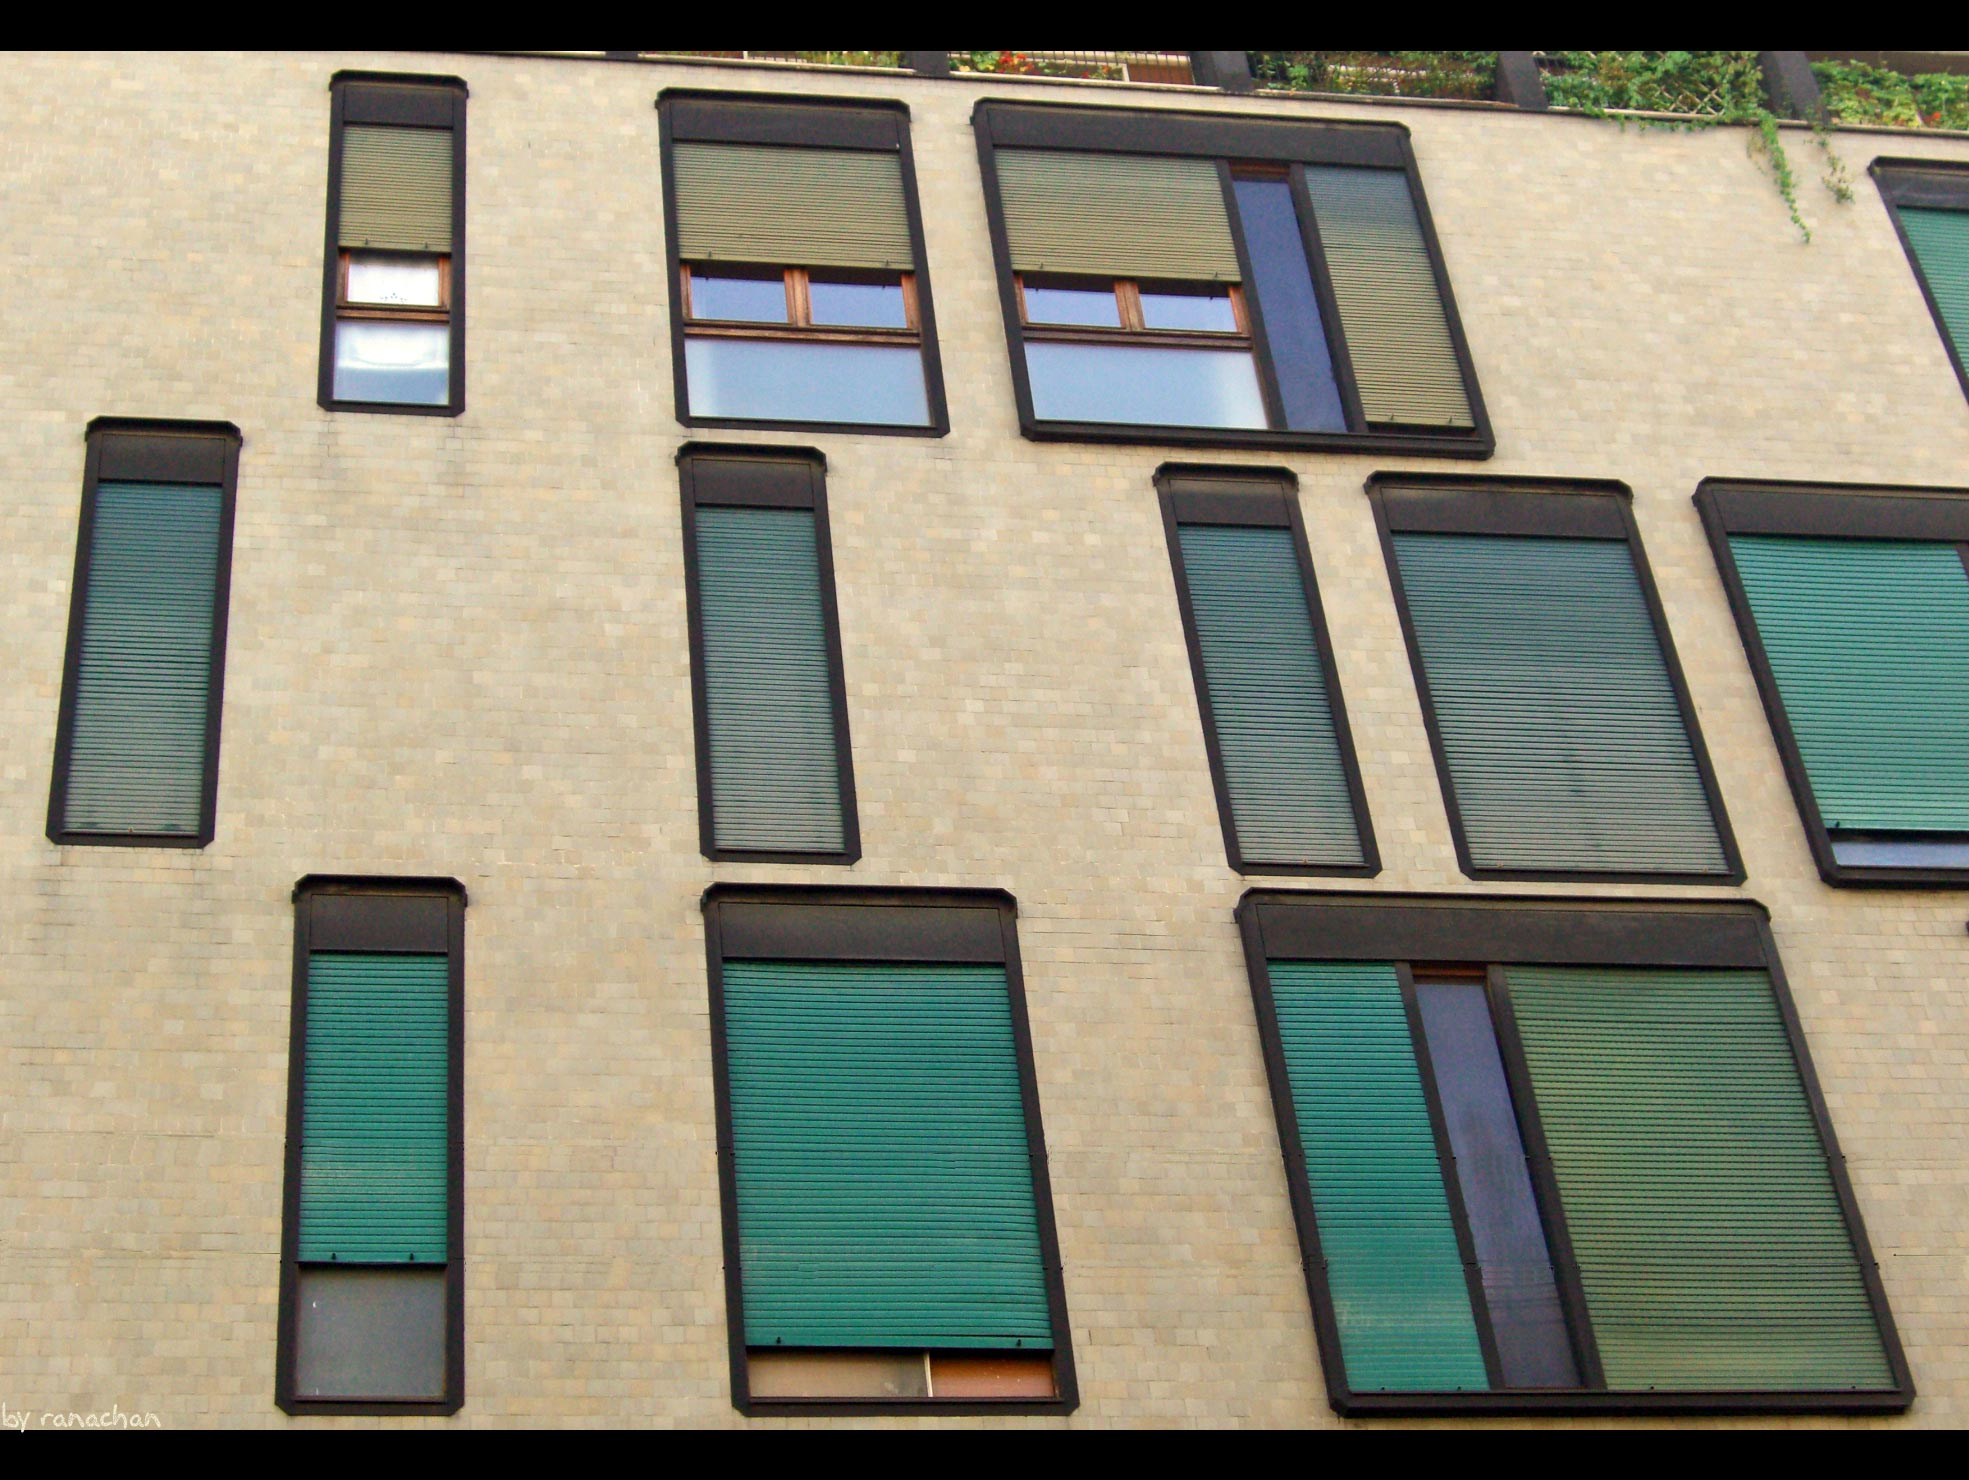
\includegraphics[width=0.95\textwidth]{\folder img/window_geometry.jpg}
%   \begin{center}
%     {\large ``Window geometry''}\par
%     Foto di midori.no.kerochan\par
%     \url{http://www.flickr.com/photos/28661972@N05/2751042868/}\par
%     Licenza: Creative Commons Attribution 2.0\par
%   \end{center}
% \newpage


\section{Estensione superficiale}
\label{sect:estensione_superficiale}

Il \emph{tangram}\label{tangram} è un antichissimo gioco cinese. Il 
nome con cui lo conosciamo si pensa derivato dall'unione della parola 
\emph{tang} o \emph{tan}, che significa \emph{cinese}, e \emph{gram} 
che significa \emph{immagine}. Anticamente in Cina era chiamato 
``schema intelligente a sette pezzi'' o anche ``le sette pietre della 
saggezza'' poiché si riteneva che la padronanza del gioco fosse la 
chiave per ottenere saggezza e talento.
Il gioco è costituito da un quadrato ritagliato in 7~pezzi poligonali 
aventi in comune solo punti del loro contorno 
(figura~\ref{fig:tangram}).


\begin{inaccessibleblock}[Figura: TODO]
 \begin{figure}[!htb]
  \centering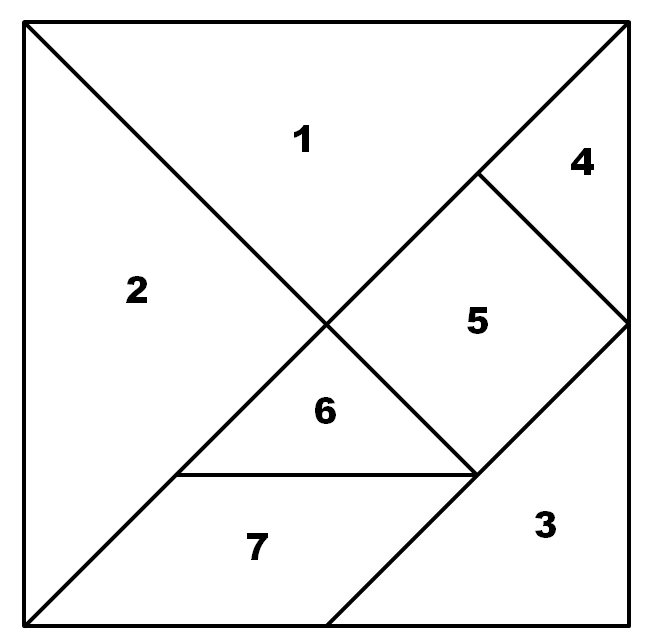
\includegraphics[width=0.6\textwidth]{\folder img/tangram.png}
  \caption{Il gioco del tangram}\label{fig:tangram}
\end{figure}
\end{inaccessibleblock}

I pezzi possono essere disposti e accostati gli uni agli altri senza 
sovrapposizioni in modo da ottenere una grande varietà di figure; la 
regola base è che devono essere utilizzati tutti i 7~pezzi. Si 
possono così formare alcuni disegni come mostrato nella 
figura~\ref{fig:figure_tangram}.


\begin{inaccessibleblock}[Figura: TODO]
 \begin{figure}[!htb]
 \centering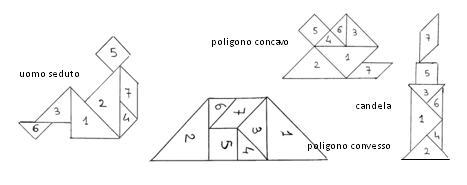
\includegraphics[width=0.8\textwidth]
    {\folder img/figure_tangram.png}
  \caption{Alcune figure realizzabili con il 
tangram}\label{fig:figure_tangram}
\end{figure}
\end{inaccessibleblock}

Potete osservare che si forma un poligono quando i singoli pezzi 
vengono accostati mediante un lato: l'uomo seduto è un poligono, ma 
non la candela; i due poligoni rappresentati sono l'uno concavo e 
l'altro convesso.

Con tutti i 7~pezzi del gioco si possono costruire 13~poligoni 
convessi, compreso il quadrato iniziale, provate a costruirli: 
fotocopiate la pagina precedente e ritagliate i 7~pezzi del tangram.

Evidentemente i 13~poligoni che avrete costruito non sono congruenti, 
né hanno la stessa forma; potete dire che sono formati dalle stesse 
parti poligonali, ciascuno può cioè essere pensato come unione dei 
\emph{tan} aventi in comune almeno un punto del loro perimetro, ma 
nessun punto interno.

\begin{definizione}
Con \emph{somma} di due \emph{figure piane} $X$ e $Y$, non aventi 
punti comuni o aventi in comune solo punti del loro contorno, 
intendiamo la figura $Z$ unione dei punti di $X$ e $Y$ e la 
indicheremo con
\begin{empheq}[box=\fbox]{equation*}
Z=X+Y
\end{empheq}
Diremo inoltre che $X$ è la \emph{differenza} tra $Z$ e $Y$ e 
scriveremo
\begin{empheq}[box=\fbox]{equation*}
X=Z-Y
\end{empheq}
\end{definizione}

\begin{definizione}
Due poligoni $p_1$ e $p_2$ sono \emph{equicomposti} se sono formati 
dalle stesse parti poligonali (figure piane). Sono 
\emph{equiscomponibili} se è possibile decomporre uno di essi in un 
numero finito di parti poligonali con le quali si possa ricoprire 
l'altro. In simboli
\begin{empheq}[box=\fbox]{equation*}
\vphantom{I}p_1 \doteq p_2
\end{empheq}
\noindent che si legge ``$p_1$ equicomposto $p_2$''
\end{definizione}

Tutte le figure poligonali costruite con i pezzi del tangram $p_1$, 
$p_2$, \ldots{} sono dunque poligoni equicomposti, ma possono anche 
essere considerati poligoni equiscomponibili, quindi $p_1 \doteq p_2 
\doteq \ldots{}$

% \begin{exrig}
\noindent\begin{minipage}{0.65\textwidth}\parindent15pt
\begin{esempio}\label{es:7.1}
Ritagliate da un quadrato i quattro triangoli rettangoli isosceli che 
si ottengono tracciando le sue diagonali (fotocopia e ritaglia la 
figura a fianco). Disponendo fianco a fianco i triangoli ottenuti in 
modo che i due lati comuni abbiano la stessa lunghezza, si ottengono 
14~figure diverse. Due di esse sono riportate nella 
figura~\ref{fig:quadrato2}. Realizzate tutte le altre figure.
\end{esempio}
\end{minipage}\hfil
\begin{minipage}{0.35\textwidth}
  \centering% Copyright (c) 2015 Daniele Masini - d.masini.it@gmail.com

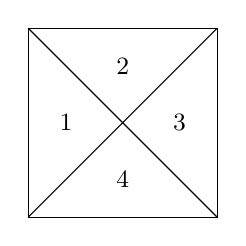
\begin{tikzpicture}[scale=1.2,font=\small]
\usetikzlibrary{calc}

\begin{scope}

\draw (0,0) -- (2,2);
\draw (0,2) -- (2,0);
\draw (0,0) -- (2,0) -- (2,2) -- (0,2) -- cycle;

\node at (0.4,1) {1};
\node at (1,1.6) {2};
\node at (1.6,1) {3};
\node at (1,0.4) {4};

\end{scope}

\end{tikzpicture}

\end{minipage}\vspace{5pt}


\begin{inaccessibleblock}[Figura: TODO]
 \begin{figure}[!htb]
\centering% Copyright (c) 2015 Daniele Masini - d.masini.it@gmail.com

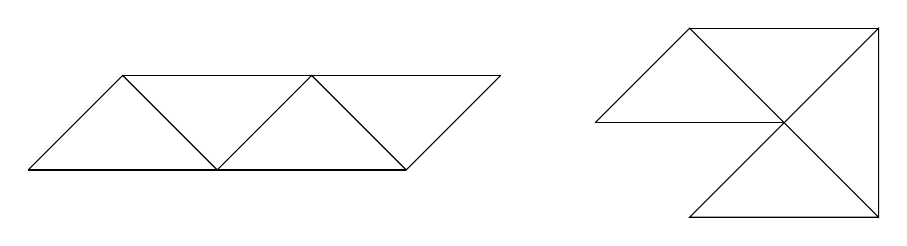
\begin{tikzpicture}[scale=1.2,font=\small]
\usetikzlibrary{calc}

\begin{scope}

\draw (0,0) -- (4,0);
\draw (1,1) -- (5,1);
\draw (0,0) -- (1,1) -- (2,0) -- (3,1) -- (4,0) -- (5,1);

\end{scope}


\begin{scope}[xshift=6cm, yshift=0.5cm]

\draw (0,0) -- (2,0);
\draw (1,1) -- (3,1);
\draw (0,0) -- (1,1) -- (2,0) -- (3,1) -- (3,-1) -- (2,0) -- (1,-1) -- (3,-1);

\end{scope}

\end{tikzpicture}

\caption{Alcune figure realizzabili 
(esempio~\ref{es:7.1})}\label{fig:quadrato2}
\end{figure}
\end{inaccessibleblock}

Le figure ottenute sono \ldots\ldots\ldots\ldots{} perché sono 
formate da \ldots\ldots\ldots\ldots{}

\noindent(da: Prova di allenamento della gara di ``Matematica senza 
frontiere'' del 9/02/1994)

% \begin{esempio}\label{es:7.2}
% Nella figura~\ref{fig:figure} sono disegnati un quadrato $ABCD$, un 
% rettangolo $PQRS$ avente $PQ=2AB$ e $SP=AB/2$ e un rombo $FGHK$ 
% avente una diagonale uguale al lato del quadrato e l'altra il doppio. 
% Mostra come sia possibile scomporre ciascuno dei tre poligoni in parti 
% tali da poter ricoprire gli altri due. Puoi concludere che i tre 
% poligoni assegnati sono equiscomponibili? \ldots\ldots{}
% 
% 
% \begin{inaccessibleblock}[Figura: TODO]
%  \begin{figure}[!htb]
%   \centering% Copyright (c) 2015 Daniele Masini - d.masini.it@gmail.com

\begin{tikzpicture}[scale=1.5,font=\small]
\usetikzlibrary{calc}

\begin{scope}
\draw (0,0) rectangle (1,1);
\node[shift={(-.2,-.2)}] at (0,0) {$A$};
\node[shift={(.2,-.2)}] at (1,0) {$D$};
\node[shift={(.2,.2)}] at (1,1) {$C$};
\node[shift={(-.2,.2)}] at (0,1) {$D$};
\end{scope}

\begin{scope}[xshift=2cm, yshift=0.25cm]
\draw (0,0) rectangle (2,0.5);
\node[shift={(-.2,-.2)}] at (0,0) {$P$};
\node[shift={(.2,-.2)}] at (2,0) {$Q$};
\node[shift={(.2,.2)}] at (2,0.5) {$R$};
\node[shift={(-.2,.2)}] at (0,0.5) {$S$};
\end{scope}

\begin{scope}[xshift=5cm, yshift=0.5cm]
\draw (0,0) node[shift={(-.2,0)}] {$F$} -- (1,-0.5) node[shift={(0,-.2)}] {$G$} -- (2,0) node[shift={(.2,0)}] {$H$} -- (1,0.5) node[shift={(0,.2)}] {$K$} -- cycle;
\end{scope}

\end{tikzpicture}

%   \caption{Esempio~\ref{es:7.2}}\label{fig:figure}
% \end{figure}
% \end{inaccessibleblock}
% 
% \end{esempio}
% 
% \noindent\begin{minipage}{0.6\textwidth}\parindent15pt
% \begin{esempio}\label{es:7.3}
% Dato l'insieme $F = \{f_1\text{,}f_2\text{,}f_3\}$ delle figure 
% poligonali disegnate a lato, segui le seguenti istruzioni:\\
% \verb|   |\textsl{ripeti:}\\
% \verb|      |\textsl{scegli una figura dell'insieme $F$;}\\
% \verb|      |\textsl{traccia alcuni segmenti che la decompongano in}\\
% \verb|        |\textsl{parti poligonali;}\\
% \verb|      |\textsl{forma con le parti ottenute altre 3 figure poligo-}\\
% \verb|        |\textsl{nali;}\\
% \verb|   |\textsl{finché non hai esaurito le figure.}\\
% Costruisci l'insieme $G$ di tutti i poligoni ottenuti con questa 
% procedura e indica con simboli arbitrari i suoi elementi.
% \end{esempio}
% \end{minipage}\hfil
% \begin{minipage}{0.4\textwidth}
%   \centering% Copyright (c) 2015 Daniele Masini - d.masini.it@gmail.com

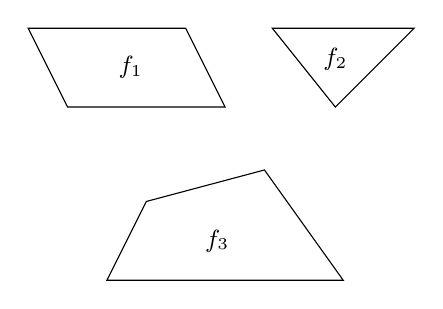
\begin{tikzpicture}[scale=2,font=\small]
\usetikzlibrary{calc}

\begin{scope}
\draw (0,0) -- (1,0) -- (0.75,0.5) -- (-0.25,0.5) -- cycle;
\node at (0.4,0.25) {$f_1$};
\end{scope}

\begin{scope}[xshift=1.7cm]
\draw (0,0) -- (0.5,0.5) -- (-0.4,0.5) -- cycle;
\node at (0,0.3) {$f_2$};
\end{scope}

\begin{scope}[xshift=0.25cm, yshift=-1.1cm]
\draw (0,0) -- (1.5,0) -- (1,0.7) -- (0.25,0.5) -- cycle;
\node at (0.7,0.25) {$f_3$};
\end{scope}

\end{tikzpicture}

% \end{minipage}\vspace{5pt}
% 
% % \end{exrig}
% 
% Nell'insieme $S=F\cup G$ (dove $F$ e $G$ sono gli insiemi definiti 
% nell'esempio~\ref{es:7.3}) la relazione $R$ espressa dal predicato: 
% <<essere equicomposti>> gode della proprietà
% \begin{itemize*}
% \item riflessiva, infatti \ldots\ldots\ldots\ldots\ldots{}
% \item simmetrica, infatti \ldots\ldots\ldots\ldots\ldots{}
% \item transitiva, infatti \ldots\ldots\ldots\ldots\ldots{}
% \end{itemize*}
% Si può dunque concludere che $R$ è una relazione di equivalenza e 
% quindi si possono costruire sia l'insieme delle parti $P(S)$, sia 
% l'insieme quoziente $E=S/R$ avente come elementi le tre classi di 
% equivalenza, ciascuna rappresentata dal poligono iniziale 
% (figura~\ref{fig:insiemi}):
% \[ [f_1] = \{x:x\text{ è un poligono equicomposto con }f_1\}; \]
% \[ [f_2] = \{x:x\text{ è un poligono equicomposto con }f_2\}; \]
% \[ [f_3] = \{x:x\text{ è un poligono equicomposto con }f_3\}. \]
% 
% 
% \begin{inaccessibleblock}[Figura: TODO]
%  \begin{figure}[!htb]
%   \centering% Copyright (c) 2015 Daniele Masini - d.masini.it@gmail.com

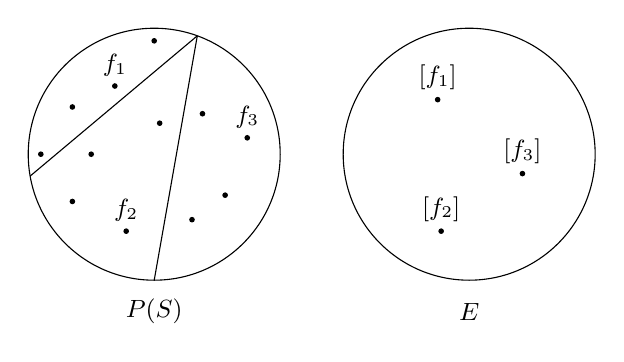
\begin{tikzpicture}[scale=0.8,font=\small]
\usetikzlibrary{calc}

\begin{scope}
\draw (0,0) circle (2);
\draw[fill] (90:1.8) circle (1pt);
\draw[fill] (120:1.25) circle (1pt)  node[above] {$f_1$};
\draw[fill] (150:1.5) circle (1pt);
\draw[fill] (180:1.8) circle (1pt);
\draw (70:2) -- (190:2);
\draw[fill] (80:0.5) circle (1pt);
\draw[fill] (180:1) circle (1pt);
\draw[fill] (210:1.5) circle (1pt);
\draw[fill] (250:1.3) circle (1pt) node[above] {$f_2$};
\draw (70:2) -- (270:2);
\draw[fill] (300:1.2) circle (1pt);
\draw[fill] (330:1.3) circle (1pt);
\draw[fill] (40:1) circle (1pt);
\draw[fill] (10:1.5) circle (1pt) node[above] {$f_3$};
\node at (0,-2.5) {$P(S)$};
\end{scope}

\begin{scope}[xshift=5cm]
\draw (0,0) circle (2);
\draw[fill] (120:1) circle (1pt) node[above] {$[f_1]$};
\draw[fill] (250:1.3) circle (1pt) node[above] {$[f_2]$};
\draw[fill] (340:0.9) circle (1pt) node[above] {$[f_3]$};
\node at (0,-2.5) {$E$};
\end{scope}

\end{tikzpicture}

%   \caption{Rappresentazione dell'insieme delle parti di $S$ e 
% del quoziente $E=S/R$}\label{fig:insiemi}
% \end{figure}
% \end{inaccessibleblock}

\begin{definizione}
Diciamo che due qualunque poligoni $p_1$ e $p_2$ appartenenti alla 
stessa classe sono \emph{equivalenti} e useremo la scrittura 
$p_1\doteq p_2$ per esprimere questa caratteristica 
(\emph{equivalenza per scomposizione}); essi hanno una caratteristica 
comune che chiamiamo \emph{estensione superficiale} (ES).
\end{definizione}

I poligoni costruiti con i pezzi del tangram appartengono alla stessa 
classe di equivalenza; essi sono dunque poligoni equivalenti e hanno 
la stessa estensione superficiale del quadrato iniziale.
Anche i 14~poligoni realizzati nell'esempio~\ref{es:7.1} appartengono 
alla stessa classe di equivalenza; essi sono dunque poligoni 
equivalenti e hanno la stessa estensione superficiale del quadrato 
assegnato.

\osservazione Sin dalla scuola elementare avete usato termini come 
``superficie'', ``estensione'' e ``area'' quando vi siete accostati 
allo studio dei poligoni, probabilmente ritenendoli sinonimi. Lo 
studio di una particolare relazione di equivalenza vi ha mostrato che 
il concetto di estensione di un poligono si ottiene attraverso il 
procedimento di passaggio al quoziente nell'insieme dei poligoni 
piani.

\begin{definizione}
Chiamiamo \emph{area} di un poligono $p$ il numero reale positivo 
$A(p)$ che esprime la misura della sua estensione superficiale.
\end{definizione}

Possiamo concludere che ad ogni classe di equivalenza, generata con 
la relazione <<essere equicomposti>> o <<essere equiscomponibili>>, 
può essere associato un numero: l'area della figura scelta come 
rappresentante della classe di equivalenza. In tal modo trasformeremo 
una relazione di equivalenza tra poligoni, espressa con il simbolo 
$\doteq$ in una relazione di uguaglianza tra numeri.
Ad esempio, riferendoci ai poligoni costruiti con i pezzi del tangram 
possiamo trasformare la relazione di equivalenza $p_1\doteq p_2\doteq 
p_3\doteq \ldots{}$ in un'uguaglianza tra le aree scrivendo 
$A(p_1)=A(p_2)=A(p_3)=\ldots{}$

\section{Poligoni equivalenti}
\label{sect:poligoni_equivalenti}

Premettiamo alcuni assiomi:
\nopagebreak
\begin{enumerate} [noitemsep]
\item Poligoni congruenti sono equivalenti.
\item Un poligono non è equivalente ad una sua parte propria.
\item Somma e differenza di poligoni equivalenti originano poligoni 
equivalenti.
\end{enumerate}

\begin{teorema}\label{teo:7.1}
Due parallelogrammi aventi rispettivamente congruenti le basi e le 
rispettive altezze, sono equivalenti.
\end{teorema}

Nella figura sottostante sono rappresentati alcuni degli infiniti 
parallelogrammi aventi basi e altezze congruenti; le loro basi 
appartengono a rette parallele.

\noindent Ipotesi: $AB\cong EF\cong IJ$, $DM\perp AB$, $HN\perp EF$, 
$LO\perp IJ$, $DM\cong HN\cong LO$.\\
Tesi: $ABCD\doteq EFGH\doteq IJLK$.\\

\begin{figure*}[!htb]
  
\centering% Copyright (c) 2015 Daniele Masini - d.masini.it@gmail.com

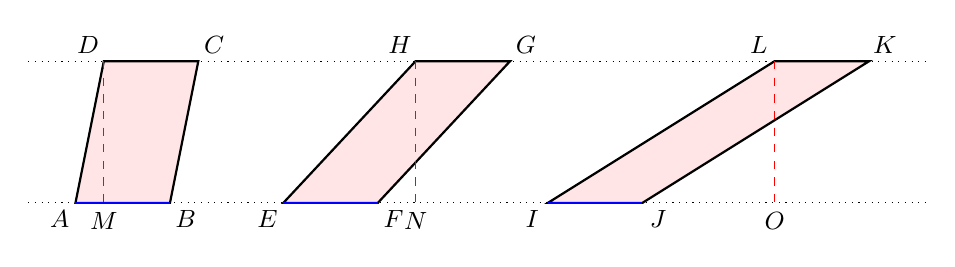
\begin{tikzpicture}[scale=1.2,font=\small]
\usetikzlibrary{calc}

\draw[dotted] (-0.5,0) -- (9,0);
\draw[dotted] (-0.5,1.5) -- (9,1.5);
\begin{scope}
\draw[thick, fill=red!10] (0,0) coordinate (a) node[shift={(-0.2,-0.2)}] {$A$} -- (1,0) coordinate (b) node[shift={(0.2,-0.2)}] {$B$} -- (1.3,1.5) coordinate (c) node[shift={(0.2,0.2)}] {$C$} -- (0.3,1.5) coordinate (d) node[shift={(-0.2,0.2)}] {$D$} -- cycle;
\draw[dashed, red] (d) -- ($(a)!(d)!(b)$) node[below, black] {$M$};
\draw[thick, blue] (a) -- (b);
\end{scope}

\begin{scope}[xshift=2.2cm]
\draw[thick, fill=red!10] (0,0) coordinate (e) node[shift={(-0.2,-0.2)}] {$E$} -- (1,0) coordinate (f) node[shift={(0.2,-0.2)}] {$F$} -- (2.4,1.5) coordinate (g) node[shift={(0.2,0.2)}] {$G$} -- (1.4,1.5) coordinate (h) node[shift={(-0.2,0.2)}] {$H$} -- cycle;
\draw[dashed, red] (h) -- ($(e)!(h)!(f)$) node[below, black] {$N$};
\draw[thick, blue] (e) -- (f);
\end{scope}

\begin{scope}[xshift=5cm]
\draw[thick, fill=red!10] (0,0) coordinate (i) node[shift={(-0.2,-0.2)}] {$I$} -- (1,0) coordinate (j) node[shift={(0.2,-0.2)}] {$J$} -- (3.4,1.5) coordinate (k) node[shift={(0.2,0.2)}] {$K$} -- (2.4,1.5) coordinate (l) node[shift={(-0.2,0.2)}] {$L$} -- cycle;
\draw[dashed, red] (l) -- ($(i)!(l)!(j)$) node[below, black] {$O$};
\draw[thick, blue] (i) -- (j);
\end{scope}

\end{tikzpicture}

\end{figure*}

Si tralascia la dimostrazione. Alcuni esempi saranno offerti con le più 
semplici dimostrazioni dei corollari.
 
\begin{corollario}\label{cor:7.1}
Ogni parallelogramma è equivalente al rettangolo avente un lato 
congruente alla sua base e l'altro lato congruente alla sua altezza.
\end{corollario}

\noindent Ipotesi: $AB\cong EF$, $CF\perp AB$, $CK\cong HE$.\\
Tesi: $ABCD\doteq EFGH$.

\begin{figure*}[!htb]
  \centering% Copyright (c) 2015 Daniele Masini - d.masini.it@gmail.com

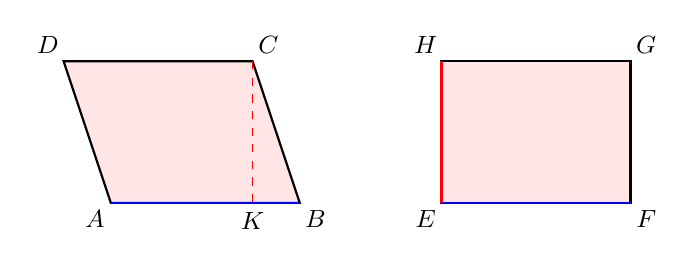
\begin{tikzpicture}[scale=1.2,font=\small]
\usetikzlibrary{calc}

\begin{scope}
\draw[thick, fill=red!10] (0,0) coordinate (a) node[shift={(-0.2,-0.2)}] {$A$} -- (2,0) coordinate (b) node[shift={(0.2,-0.2)}] {$B$} -- (1.5,1.5) coordinate (c) node[shift={(0.2,0.2)}] {$C$} -- (-0.5,1.5) coordinate (d) node[shift={(-0.2,0.2)}] {$D$} -- cycle;
\draw[dashed, red] (c) -- ($(a)!(c)!(b)$) node[below, black] {$K$};
\draw[thick, blue] (a) -- (b);
\end{scope}

\begin{scope}[xshift=3.5cm]
\draw[thick, fill=red!10] (0,0) coordinate (e) node[shift={(-0.2,-0.2)}] {$E$} -- (2,0) coordinate (f) node[shift={(0.2,-0.2)}] {$F$} -- (2,1.5) coordinate (g) node[shift={(0.2,0.2)}] {$G$} -- (0,1.5) coordinate (h) node[shift={(-0.2,0.2)}] {$H$} -- cycle;
\draw[thick, red] (e) -- (h);
\draw[thick, blue] (e) -- (f);
\end{scope}

\end{tikzpicture}

\end{figure*}

\noindent\begin{minipage}{0.65\textwidth}\parindent15pt
\begin{proof}
Dal vertice $D$ tracciamo l'altezza $DL$ relativa alla base $AB$; il 
quadrilatero $DLKC$ è un rettangolo congruente a $EFGH$; dimostrando 
che $ABCD\doteq DLKC$ si ottiene la tesi.\\
Completate la dimostrazione.\\
Osserviamo che $ABCD$ è composto da \ldots\ldots\ldots\ldots{}
e $DLKC$ è composto da \ldots\ldots\ldots\ldots{} 
Consideriamo i triangoli \ldots\ldots\ldots\ldots{}
Sono congruenti perché \ldots\ldots\ldots\ldots{}
quindi \ldots\ldots\ldots\ldots{}
\end{proof}
\end{minipage}\hfil
\begin{minipage}{0.35\textwidth}
  \centering% Copyright (c) 2015 Daniele Masini - d.masini.it@gmail.com

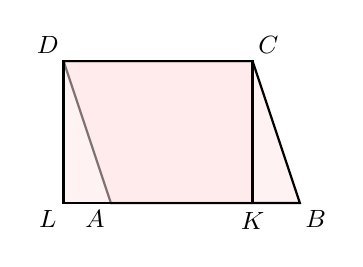
\begin{tikzpicture}[scale=1.2,font=\small]
\usetikzlibrary{calc}

\begin{scope}
\path[fill=red!10, opacity=0.5] (0,0) coordinate (a) -- (2,0) coordinate (b) -- (1.5,1.5) coordinate (c) -- (-0.5,1.5) coordinate (d) -- cycle;
\draw[thick] (a) node[shift={(-0.2,-0.2)}] {$A$} -- (b) node[shift={(0.2,-0.2)}] {$B$} -- (c) node[shift={(0.2,0.2)}] {$C$} -- (d) node[shift={(-0.2,0.2)}] {$D$} -- cycle;
\node[below] at ($(a)!(c)!(b)$) {$K$};
\end{scope}

\begin{scope}[xshift=-.5cm]
\path[fill=red!10, opacity=0.5] (0,0) coordinate (e) -- (2,0) coordinate (f) -- (2,1.5) coordinate (g) -- (0,1.5) coordinate (h) -- cycle;
\draw[thick] (e) node[shift={(-0.2,-0.2)}] {$L$} -- (f) -- (g) -- (h) -- cycle;
\end{scope}

\end{tikzpicture}

\end{minipage}\vspace{5pt}

Il teorema~\ref{teo:7.1} e il suo corollario~\ref{cor:7.1} ci 
assicurano che i parallelogrammi aventi rispettivamente congruenti le 
basi e le relative altezze formano una classe di equivalenza avente 
come rappresentante il rettangolo che ha un lato congruente alla base 
del parallelogramma e l'altro lato congruente alla sua altezza. 
Possiamo quindi affermare che $ABCD\doteq EFGH \:\Rightarrow\: 
A_{ABCD} = A_{EFGH}$.

\begin{teorema}\label{teo:7.2}
Un triangolo è equivalente ad un parallelogramma avente:
\begin{enumeratea}
\item base congruente alla metà della base del triangolo e altezza 
congruente all'altezza del triangolo, oppure
\item base congruente alla base del triangolo e altezza congruente 
alla metà dell'altezza del triangolo.
\end{enumeratea}
\end{teorema}

Nella figura sono rappresentati il triangolo $ABC$, il 
parallelogramma $DEFG$ avente base congruente alla metà della base del 
triangolo e altezza congruente all'altezza del triangolo, il 
parallelogramma $IJLM$ avente altezza congruente alla metà 
dell'altezza del triangolo e base congruente alla base del triangolo.

\noindent Ipotesi: $AB\perp CH$, $DE\cong \frac{1}{2}AB$, $GK\perp 
DE$, $GK\cong CH$, $IJ\cong AB$, $MN\perp IJ$, $MN\cong 
\frac{1}{2}CH$.\\
Tesi: a) $ABC\doteq DEFG$;\quad b) $ABC\doteq IJLM$.

\begin{figure*}[!htb]
  \centering% Copyright (c) 2015 Daniele Masini - d.masini.it@gmail.com

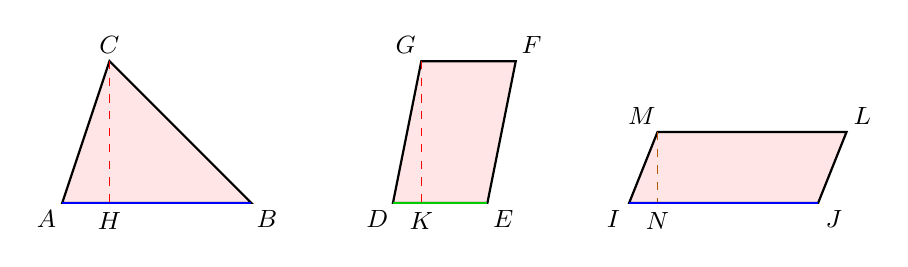
\begin{tikzpicture}[scale=1.2,font=\small]
\usetikzlibrary{calc}

\begin{scope}
\draw[thick, fill=red!10] (0,0) coordinate (a) node[shift={(-0.2,-0.2)}] {$A$} -- (2,0) coordinate (b) node[shift={(0.2,-0.2)}] {$B$} -- (0.5,1.5) coordinate (c) node[shift={(0,0.2)}] {$C$} -- cycle;
\draw[dashed, red] (c) -- ($(a)!(c)!(b)$) node[below, black] {$H$};
\draw[thick, blue] (a) -- (b);
\end{scope}

\begin{scope}[xshift=3.5cm]
\draw[thick, fill=red!10] (0,0) coordinate (d) node[shift={(-0.2,-0.2)}] {$D$} -- (1,0) coordinate (e) node[shift={(0.2,-0.2)}] {$E$} -- (1.3,1.5) coordinate (f) node[shift={(0.2,0.2)}] {$F$} -- (0.3,1.5) coordinate (g) node[shift={(-0.2,0.2)}] {$G$} -- cycle;
\draw[dashed, red] (g) -- ($(d)!(g)!(e)$) node[below, black] {$K$};
\draw[thick, green!80!black] (d) -- (e);
\end{scope}

\begin{scope}[xshift=6cm]
\draw[thick, fill=red!10] (0,0) coordinate (i) node[shift={(-0.2,-0.2)}] {$I$} -- (2,0) coordinate (j) node[shift={(0.2,-0.2)}] {$J$} -- (2.3,0.75) coordinate (l) node[shift={(0.2,0.2)}] {$L$} -- (0.3,0.75) coordinate (m) node[shift={(-0.2,0.2)}] {$M$} -- cycle;
\draw[dashed, orange!70!black] (m) -- ($(i)!(m)!(j)$) node[below, black] {$N$};
\draw[thick, blue] (i) -- (j);
\end{scope}

\end{tikzpicture}

\end{figure*}

\begin{proof}~\vspace{4pt}\\
\noindent\begin{minipage}{0.65\textwidth}\parindent15pt
\noindent\emph{Caso a.}\\
Dal punto medio $T$ della base $AB$ tracciamo la parallela al lato 
$AC$ che incontra $CB$ in $S$; dal vertice $C$ tracciamo la parallela 
alla base $AB$ che interseca in $R$ la retta $ST$; il parallelogramma 
$ATRC$ soddisfa le ipotesi del caso a) ed è equivalente a $DEFG$ per 
il teorema~\ref{teo:7.1}.
Confrontiamo il triangolo e il parallelogramma: possiamo pensare 
$ABC$ composto da $CATS+BST$ e $ATRC$ composto da $CATS+CSR$.
\end{minipage}\hfil
\begin{minipage}{0.35\textwidth}
  \centering% Copyright (c) 2015 Daniele Masini - d.masini.it@gmail.com

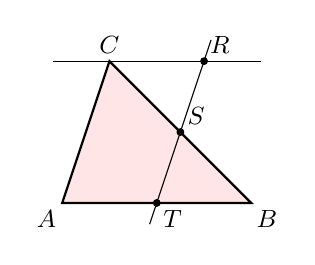
\begin{tikzpicture}[scale=1.2,font=\small]
\usetikzlibrary{calc}

\begin{scope}
\draw[thick, fill=red!10] (0,0) coordinate (a) node[shift={(-0.2,-0.2)}] {$A$} -- (2,0) coordinate (b) node[shift={(0.2,-0.2)}] {$B$} -- (0.5,1.5) coordinate (c) node[shift={(0,0.2)}] {$C$} -- cycle;
%\draw[dashed, red] (c) -- ($(a)!(c)!(b)$) node[below, black] {$H$};
\draw (-0.1,1.5) coordinate (r1) -- (2.1,1.5) coordinate (r2);
\coordinate (t) at ($(a)!0.5!(b)$);
\coordinate (s) at ($(b)!0.5!(c)$);
\draw ($(t)!-0.3!(s)$) -- ($(t)!2.3!(s)$);
\coordinate (r) at (intersection of s--t and r1--r2);
\draw[fill] (r) circle (1pt) node[shift={(0.2,0.2)}] {$R$};
\draw[fill] (s) circle (1pt) node[shift={(0.2,0.2)}] {$S$};
\draw[fill] (t) circle (1pt) node[shift={(0.2,-0.2)}] {$T$};

\end{scope}

\end{tikzpicture}

\end{minipage}\vspace{1pt}
Se dimostriamo la congruenza dei triangoli $CSR$ e $BST$ potremo 
concludere che triangolo e parallelogramma, essendo equicomposti, 
sono equivalenti. 
$TB\cong CR$ infatti \ldots\ldots\ldots\ldots{}
$SB\cong CS$ infatti \ldots\ldots\ldots\ldots{}
$T\widehat{B}S\cong S\widehat{C}R$ infatti \ldots\ldots\ldots\ldots{}
Allora per il primo criterio di congruenza $TBS\cong SCR$ e quindi 
$ATRC\doteq BST$.\\

\noindent\begin{minipage}{0.65\textwidth}\parindent15pt
\noindent\emph{Caso b.}\\
Dal punto medio $V$ dell'altezza $CH$ tracciamo la parallela alla 
base $AB$ che interseca i lati $AC$ e $BC$ rispettivamente in $W$ e 
$Z$; da $B$ tracciamo la parallela al lato $AC$ che interseca la retta 
$WZ$ in $U$; il parallelogramma $AWUB$ soddisfa le ipotesi del caso b) 
ed è equivalente a $IJLM$ per il teorema~\ref{teo:7.1}.
Confrontiamo il triangolo e il parallelogramma: possiamo pensare 
$ABC$ composto da \ldots\ldots\ldots{} e $AWUB$ composto da 
\ldots\ldots\ldots{}
Se dimostriamo la congruenza dei triangoli $CWZ$ e $ZBU$ potremo 
concludere che triangolo e parallelogramma, essendo equicomposti, 
sono equivalenti.
$CW\cong \ldots{}$ infatti \ldots\ldots\ldots\ldots{}
$CZ\cong \ldots{}$ infatti \ldots\ldots\ldots\ldots{}
$\ldots{}\cong Z\widehat{B}U$ infatti \ldots\ldots\ldots\ldots{}
Pertanto \ldots\ldots\ldots\ldots{}
\end{minipage}\hfil
\begin{minipage}{0.35\textwidth}
  \centering% Copyright (c) 2015 Daniele Masini - d.masini.it@gmail.com

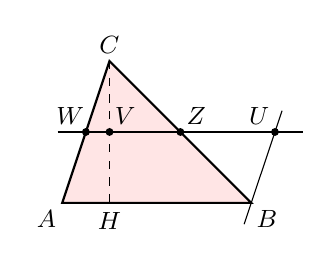
\begin{tikzpicture}[scale=1.2,font=\small]
\usetikzlibrary{calc}

\begin{scope}
\draw[thick, fill=red!10] (0,0) coordinate (a) node[shift={(-0.2,-0.2)}] {$A$} -- (2,0) coordinate (b) node[shift={(0.2,-0.2)}] {$B$} -- (0.5,1.5) coordinate (c) node[shift={(0,0.2)}] {$C$} -- cycle;
\draw[dashed] (c) -- ($(a)!(c)!(b)$) coordinate (h) node[below, black] {$H$};
\coordinate (t) at ($(a)!0.5!(b)$);
\coordinate (z) at ($(b)!0.5!(c)$);
\coordinate (w) at ($(a)!0.5!(c)$);
\path (b) -- +($(z)-(t)$) coordinate (b1);

\coordinate (u) at (intersection of w--z and b--b1);
\coordinate (v) at (intersection of c--h and w--z);

\draw ($(b)!-0.3!(u)$) -- ($(b)!1.3!(u)$);
\draw ($(w)!-0.3!(z)$) -- ($(w)!2.3!(z)$);

\draw[fill] (w) circle (1pt) node[shift={(-0.2,0.2)}] {$W$};
\draw[fill] (z) circle (1pt) node[shift={(0.2,0.2)}] {$Z$};
\draw[fill] (u) circle (1pt) node[shift={(-0.2,0.2)}] {$U$};
\draw[fill] (v) circle (1pt) node[shift={(0.2,0.2)}] {$V$};

\end{scope}

\end{tikzpicture}

\end{minipage}\vspace{1pt}
\end{proof}

\begin{corollario}\label{cor:7.2}
I triangoli aventi la stessa base e la stessa altezza sono 
equivalenti.
\end{corollario}

Lasciamo al lettore la dimostrazione di questa proprietà.

\begin{wrapfigure}{r}{0.6\textwidth}
  \centering% Copyright (c) 2015 Daniele Masini - d.masini.it@gmail.com

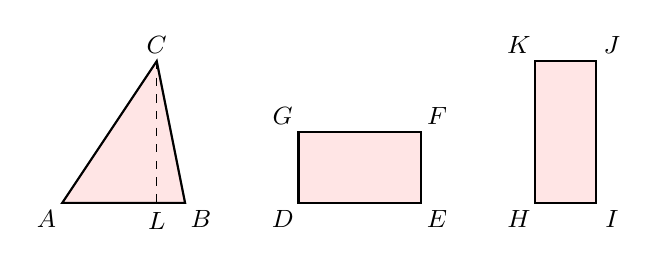
\begin{tikzpicture}[scale=1.2,font=\small]
\usetikzlibrary{calc}

\begin{scope}
\draw[thick, fill=red!10] (0,0) coordinate (a) node[shift={(-0.2,-0.2)}] {$A$} -- (1.3,0) coordinate (b) node[shift={(0.2,-0.2)}] {$B$} -- (1,1.5) coordinate (c) node[shift={(0,0.2)}] {$C$} -- cycle;
\draw[dashed] (c) -- ($(a)!(c)!(b)$) coordinate (l) node[below, black] {$L$};
\end{scope}

\begin{scope}[xshift=2.5cm]
\draw[thick, fill=red!10] (0,0) coordinate (d) node[shift={(-0.2,-0.2)}] {$D$} -- (1.3,0) coordinate (e) node[shift={(0.2,-0.2)}] {$E$} -- (1.3,0.75) coordinate (f) node[shift={(0.2,0.2)}] {$F$} -- (0,0.75) coordinate (g) node[shift={(-0.2,0.2)}] {$G$} -- cycle;
\end{scope}

\begin{scope}[xshift=5cm]
\draw[thick, fill=red!10] (0,0) coordinate (h) node[shift={(-0.2,-0.2)}] {$H$} -- (0.65,0) coordinate (i) node[shift={(0.2,-0.2)}] {$I$} -- (0.65,1.5) coordinate (j) node[shift={(0.2,0.2)}] {$J$} -- (0,1.5) coordinate (k) node[shift={(-0.2,0.2)}] {$K$} -- cycle;
\end{scope}


\end{tikzpicture}
\end{wrapfigure}
Il teorema~\ref{teo:7.2} e il suo corollario (\ref{cor:7.2}) ci 
assicurano che i triangoli aventi rispettivamente congruenti la base 
e la rispettiva altezza formano una classe di equivalenza avente come 
rappresentante il rettangolo con un lato congruente alla base del 
triangolo e l'altro lato congruente a metà della sua altezza, oppure 
un lato congruente all'altezza del triangolo e l'altro lato 
congruente a metà della base. 

\noindent Ipotesi: $CL\perp AB$, $DE\cong AB$, $DG\cong 
\frac{1}{2}CL$, $KH\cong CL$, $HI\cong\frac{1}{2}AB$.\\
Tesi: $ABC\doteq DEFG\doteq HIJK \:\Rightarrow\: 
A_{ABC}=A_{DEFG}=A_{HIJK}$.

\begin{teorema}\label{teo:7.3}
Un trapezio è equivalente a un triangolo avente per base la somma 
delle basi del trapezio e per altezza la stessa altezza.
\end{teorema}

\noindent Ipotesi: $EF\cong AB+CD$, $DH\perp AB$, $GI\perp EF$, 
$GI\cong DH$.\\
Tesi: $ABCD\doteq EFG$.

\begin{figure*}[!htb]
  \centering% Copyright (c) 2015 Daniele Masini - d.masini.it@gmail.com

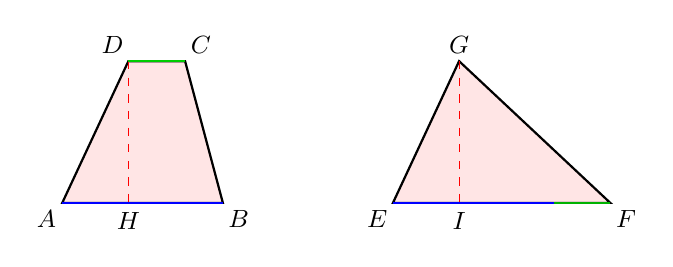
\begin{tikzpicture}[scale=1.2,font=\small]
\usetikzlibrary{calc}

\begin{scope}[xshift=2.5cm]
\draw[thick, fill=red!10] (0,0) coordinate (a) node[shift={(-0.2,-0.2)}] {$A$} -- (1.7,0) coordinate (b) node[shift={(0.2,-0.2)}] {$B$} -- (1.3,1.5) coordinate (c) node[shift={(0.2,0.2)}] {$C$} -- (0.7,1.5) coordinate (d) node[shift={(-0.2,0.2)}] {$D$} -- cycle;
\draw[dashed, red] (d) -- ($(a)!(d)!(b)$) coordinate (h) node[below, black] {$H$};
\draw[thick, blue] (a) -- (b);
\draw[thick, green!80!black] (c) -- (d);
\end{scope}

\begin{scope}[xshift=6cm]
\draw[thick, fill=red!10] (0,0) coordinate (e) node[shift={(-0.2,-0.2)}] {$E$} -- (2.3,0) coordinate (f) node[shift={(0.2,-0.2)}] {$F$} -- (0.7,1.5) coordinate (g) node[shift={(0,0.2)}] {$G$} -- cycle;
\draw[dashed, red] (g) -- ($(e)!(g)!(f)$) coordinate (j) node[below, black] {$I$};

\draw[thick, blue] (e) -- +(0:1.7) coordinate (x);
\draw[thick, green!70!black] (x) -- (f);

\end{scope}

\end{tikzpicture}

\end{figure*}

\noindent\begin{minipage}{0.65\textwidth}\parindent15pt
\begin{proof}
Prolunghiamo la base $AB$ del segmento $BP$ congruente a $DC$ e 
congiungiamo $D$ con $P$.
$APD$ è un triangolo equivalente a $EFG$ avendo stessa base e stessa 
altezza, quindi basta dimostrare che $ABCD\doteq APD$.
Confrontiamo il trapezio e il triangolo: possiamo pensare 
$ABCD$ composto da \ldots\ldots\ldots\ldots{} 
e $APD$ composto da \ldots\ldots\ldots\ldots{}
Se dimostriamo la congruenza dei triangoli \ldots\ldots\ldots\ldots{}
potremo concludere che trapezio e triangolo, essendo equicomposti, 
sono equivalenti. 
I due triangoli sono congruenti perché hanno 
\ldots\ldots\ldots\ldots{} 
Possiamo quindi affermare che $ABCD\doteq APD \:\Rightarrow\: 
A_{ABCD}=A_{APD}$.
\end{proof}
\end{minipage}\hfil
\begin{minipage}{0.35\textwidth}
  \centering% Copyright (c) 2015 Daniele Masini - d.masini.it@gmail.com

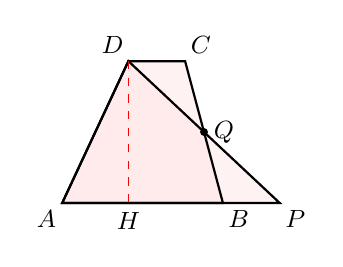
\begin{tikzpicture}[scale=1.2,font=\small]
\usetikzlibrary{calc}

\begin{scope}[xshift=2.5cm]

\path[fill=red!10, opacity=0.5] (0,0) coordinate (a) -- (1.7,0) coordinate (b) -- (1.3,1.5) coordinate (c) -- (0.7,1.5) coordinate (d) -- cycle;

\path[fill=red!10, opacity=0.5] (0,0) coordinate (e) -- (2.3,0) coordinate (f) -- (0.7,1.5) coordinate (g) -- cycle;

\draw[thick] (a) node[shift={(-0.2,-0.2)}] {$A$} -- (b) node[shift={(0.2,-0.2)}] {$B$} -- (c) node[shift={(0.2,0.2)}] {$C$} -- (d) node[shift={(-0.2,0.2)}] {$D$} -- cycle;

\draw[thick] (e) -- (f) node[shift={(0.2,-0.2)}] {$P$} -- (g) -- cycle;

\draw[dashed, red] (d) -- ($(a)!(d)!(b)$) coordinate (h) node[below, black] {$H$};

\coordinate (q) at (intersection of f--g and b--c);
\draw[fill] (q) circle (1pt) node[right] {$Q$};

\end{scope}

\end{tikzpicture}

\end{minipage}\vspace{8pt}

Pertanto, utilizzando il teorema~\ref{teo:7.2} e il suo corollario 
(\ref{cor:7.2}) possiamo sempre determinare il rettangolo equivalente 
a un trapezio dato.


\section{Aree dei principali poligoni}
\label{sect:aree_poligoni}

Per \emph{area} di una qualunque figura piana intendiamo il numero 
reale che esprime la misura dell'estensione superficiale della figura 
data.

Per calcolare le aree dei principali poligoni si ricava per prima 
l'area del rettangolo e poi, basandosi sui teoremi relativi 
all'equivalenza delle figure piane, da questa si ricavano le aree di 
altri poligoni fondamentali.

\subsection{Area del rettangolo}

\begin{teorema}
L'area del rettangolo è data dal prodotto della misura delle sue 
dimensioni
\begin{empheq}[box=\fbox]{equation*}
A=b\cdot h
\end{empheq}
\end{teorema}

\begin{figure*}[!htb]
  \centering% Copyright (c) 2015 Daniele Masini - d.masini.it@gmail.com

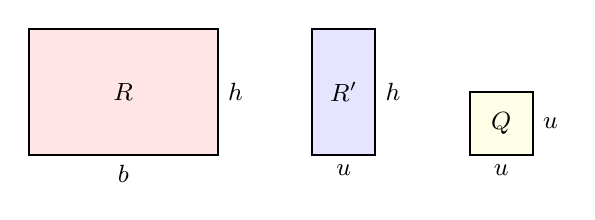
\begin{tikzpicture}[scale=0.8,font=\small]
\usetikzlibrary{calc}

\begin{scope}
\draw[thick, fill=red!10] (0,0) -- node[below] {$b$} (3,0) -- node[right] {$h$} (3,2) -- (0,2) -- cycle;
\node at (1.5,1) {$R$};
\end{scope}

\begin{scope}[xshift=4.5cm]
\draw[thick, fill=blue!10] (0,0) -- node[below] {$u$} (1,0) -- node[right] {$h$} (1,2) -- (0,2) -- cycle;
\node at (0.5,1) {$R'$};
\end{scope}

\begin{scope}[xshift=7cm]
\draw[thick, fill=yellow!10] (0,0) -- node[below] {$u$} (1,0) -- node[right] {$u$} (1,1) -- (0,1) -- cycle;
\node at (0.5,0.5) {$Q$};
\end{scope}


\end{tikzpicture}
\end{figure*}


\subsection{Area del quadrato}

Poiché il quadrato è un particolare rettangolo avente le dimensioni 
congruenti tra loro, $b = h = l$, anche la sua area si calcolerà in 
modo analogo a quella del rettangolo $A=b\cdot h=l\cdot l$ ovvero
\begin{empheq}[box=\fbox]{equation*}
A=l^2
\end{empheq}
Dunque l'area del quadrato è data dal quadrato del lato.

\subsection{Area del parallelogramma}

\begin{wrapfigure}{r}{0.3\textwidth}
  \centering% Copyright (c) 2015 Daniele Masini - d.masini.it@gmail.com

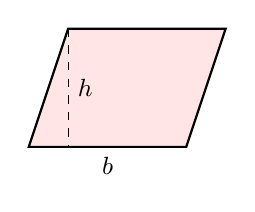
\begin{tikzpicture}[scale=1,font=\small]
\usetikzlibrary{calc}

\begin{scope}
\draw[thick, fill=red!10] (0,0) coordinate (a) -- node [below] {$b$} (2,0) coordinate (b) -- (2.5,1.5) -- (0.5,1.5) coordinate (d) -- cycle;
\draw[dashed] (d) -- node[right] {$h$} ($(a)!(d)!(b)$);
\end{scope}

\end{tikzpicture}

\end{wrapfigure}
Ricordando il teorema~\ref{teo:7.1} sull'equivalenza tra 
parallelogrammi, secondo il quale due parallelogrammi sono 
equivalenti quando hanno un lato (base) e l'altezza ad esso relativa 
tra loro congruenti, da cui deriva il corollario~\ref{cor:7.1} che un 
parallelogramma è equivalente ad un rettangolo avente base ed altezza 
congruenti a quelle del parallelogramma stesso, è immediato dedurre 
che anche l'area del parallelogramma si calcola moltiplicando un 
lato, ritenuto la base, per l'altezza ad esso relativa, cioè
\begin{empheq}[box=\fbox]{equation*}
A=b\cdot h
\end{empheq}

\subsection{Area del triangolo}

Anche in questo caso ci si deve rifare al teorema~\ref{teo:7.2} 
sull'equivalenza tra un triangolo e un parallelogramma <<Un triangolo 
è equivalente ad un parallelogramma avente come base metà della base 
del triangolo ed altezza congruente a quella del triangolo>>. Appare 
allora evidente che l'area del triangolo è
\begin{empheq}[box=\fbox]{equation*}
A=\dfrac{b}{2}\cdot h
\end{empheq}
dove $b/2$ è la base del parallelogramma ad esso equivalente.

\subsection{Area del trapezio}

Sempre dai teoremi sull'equivalenza, sappiamo che <<Un trapezio è 
equivalente ad un triangolo la cui base è congruente alla somma delle 
basi del trapezio e la cui altezza ad essa relativa è congruente 
all'altezza del trapezio>> (teorema~\ref{teo:7.3}). Dunque l'area del 
trapezio sarà
\begin{empheq}[box=\fbox]{equation*}
A=\dfrac{B+b}{2}\cdot h
\end{empheq}
dove $B + b$ è la somma delle basi del trapezio, e quindi $(B + b)/2$ 
è la base del triangolo ad esso equivalente.

\subsection{Area del rombo}

\begin{wrapfigure}{r}{0.4\textwidth}
  \centering% Copyright (c) 2015 Daniele Masini - d.masini.it@gmail.com

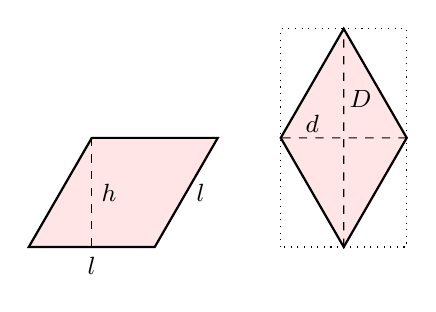
\begin{tikzpicture}[scale=0.8,font=\small]
\usetikzlibrary{calc}

\begin{scope}
\draw[thick, fill=red!10] (0,0) coordinate (a) -- node [below] {$l$} ++(0:2) coordinate (b) -- node[right] {$l$} ++(60:2) -- ++(180:2) coordinate (d) -- cycle;
\draw[dashed] (d) -- node[right] {$h$} ($(a)!(d)!(b)$);
\end{scope}

\begin{scope}[xshift=5cm]
\draw[dotted] (-1,0) rectangle (1,{sqrt(3)*2});

\begin{scope}[rotate=60]
\draw[thick, fill=red!10] (0,0) coordinate (a) -- ++(0:2) coordinate (b) -- ++(60:2) coordinate (c) -- ++(180:2) coordinate (d) -- cycle;
\draw[dashed] (a) -- node[right, shift={(-0.05,0.5)}] {$D$} (c);
\draw[dashed] (b) -- node[above, shift={(-0.4,-0.05)}] {$d$} (d);
\end{scope}
\end{scope}

\end{tikzpicture}

\end{wrapfigure}
Poiché il rombo è un particolare parallelogramma, la sua area si 
trova moltiplicando uno dei suoi lati per l'altezza ad esso relativa, 
cioè $A=l\cdot h$.
Possiamo però notare che un rombo si può considerare come la metà di 
un rettangolo le cui dimensioni sono congruenti alle diagonali del 
rombo ($D$ e $d$).
Come si può facilmente dimostrare, le due diagonali dividono il rombo 
in quattro triangoli rettangoli congruenti ai quattro triangoli 
rettangoli esterni al rombo, e quindi il rombo è equivalente alla 
metà del rettangolo, per cui la sua area può essere espressa come
\begin{empheq}[box=\fbox]{equation*}
A=\dfrac{D\cdot d}{2}
\end{empheq}

Si può inoltre dimostrare, in maniera del tutto analoga a quanto 
precedentemente descritto, che l'area di un qualsiasi quadrilatero 
che abbia le diagonali perpendicolari è determinabile in questo modo.


\section{Teoremi di Pitagora e di Euclide}
\label{sect:teoremi_pitagora_euclide}

\begin{teorema}[Primo teorema di Euclide]
In un triangolo rettangolo, il quadrato costruito su un cateto è 
equivalente al rettangolo che ha come dimensioni l'ipotenusa e la 
proiezione del cateto stesso sull'ipotenusa.
\end{teorema}


\noindent\begin{minipage}{0.63\textwidth}\parindent15pt
\begin{proof}
Sia $ABC$ un triangolo rettangolo in $B$. Tracciamo l'altezza $BH$ 
relativa all'ipotenusa $AC$ e prolunghiamola di un segmento $HD$ 
congruente all'ipotenusa stessa e costruiamo il rettangolo $AEDH$. 
Sul cateto $AB$ costruiamo il quadrato $ABGF$. Prolunghiamo i lati 
$HD$ ed $AE$ del rettangolo ed il lato $FG$ del quadrato e chiamiamo 
$I$ e $J$ i punti di intersezione tra questi prolungamenti. Otteniamo 
il parallelogramma $ABJI$.
La tesi da dimostrare è che il quadrato $ABGF$ è equivalente al 
rettangolo $AEDH$.

Consideriamo innanzitutto i triangoli $AIF$ e $ABC$, essi sono 
congruenti in quanto hanno entrambi un angolo retto ($A\widehat{F}I$ 
e $A\widehat{B}C$), $AF\cong AB$ in quanto lati di un quadrato, 
$F\widehat{A}I\cong B\widehat{A}C$ in quanto complementari dello 
stesso angolo $I\widehat{A}B$.
Dunque i due triangoli sono congruenti per il secondo criterio 
generalizzato, ed in particolare avranno $AI\cong AC$.

Consideriamo ora il parallelogramma $ABJI$ ed il quadrato $ABGF$; 
essi sono equivalenti in quanto hanno il lato $AB$ in comune e la 
stessa altezza $BG$ relativa a questo lato. 
Consideriamo poi il parallelogramma $ABJI$ ed il rettangolo $AHDE$; 
anch'essi sono equivalenti poiché hanno basi congruenti $AE$ e $AI$, 
entrambe congruenti ad $AC$, e stessa altezza $AH$.
Allora per la proprietà transitiva dell'equivalenza avremo che anche 
il quadrato $ABGF$ è equivalente al rettangolo $AEDH$ e così la tesi 
è provata.
\end{proof}
\end{minipage}\hfil
\begin{minipage}{0.37\textwidth}
  \centering% Copyright (c) 2015 Daniele Masini - d.masini.it@gmail.com

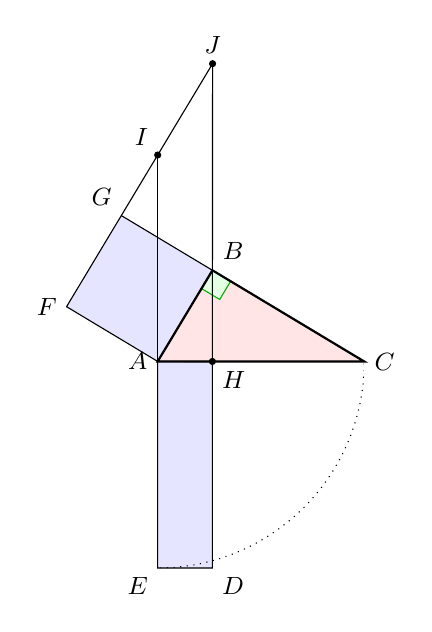
\begin{tikzpicture}[scale=0.9,font=\small]
\usetikzlibrary{calc}

%\begin{scope}[rotate=121]
\begin{scope}[rotate=-121]
\path[fill=red!10] (0,0) coordinate (a) -- (-1.5,0) coordinate (b) -- (-1.5,2.5) coordinate (c) -- cycle;
\draw[green!70!black, fill=green!10] (b) rectangle +(0.3,0.3);
\draw[fill=blue!10] (a) let \p1=(b) in -- (b) -- (\x1,\x1) coordinate (g) node[above left] {$G$} -- (0,\x1) coordinate (f) node [left] {$F$} -- cycle;
\end{scope}
\draw (b) -- ($(a)!(b)!(c)$) coordinate (h);
\draw[fill=blue!10] (a) let \p1=(c) in -- (0,{-\x1}) coordinate (e) node[below left] {$E$} let \p2=(h) in -- +({\x2},0) coordinate (d) node[below right] {$D$} -- (h) -- cycle;
\begin{scope}
\clip (a) let \p1=(c) in -- ({\x1+0.1},0) -- ({\x1},{-\x1}) -- (0,{-\x1}) -- cycle;
\draw[dotted] (a) let \p1=(c) in circle ({\x1});
\end{scope}

\draw[thick] (a) node[left] {$A$} -- (b) node [above right]{$B$} -- (c) node[right] {$C$} -- cycle;

\path (a) -- (0,1) coordinate (a1);
\coordinate (i) at (intersection of a--a1 and f--g);
\coordinate (j) at (intersection of h--b and f--g);
\draw (g) -- (j);
\draw (a) -- (i);
\draw (b) -- (j);

\draw[fill] (h) circle (1.2pt) node[below right] {$H$};
\draw[fill] (i) circle (1.2pt) node[above left] {$I$};
\draw[fill] (j) circle (1.2pt) node[above] {$J$};
%\end{scope}

\end{tikzpicture}

\end{minipage}\vspace{8pt}


\begin{teorema}[di Pitagora]
In un triangolo rettangolo il quadrato costruito sull'ipotenusa è 
equivalente alla somma dei quadrati costruiti sui cateti.
\end{teorema}

\noindent\begin{minipage}{0.55\textwidth}\parindent15pt
\begin{proof}
Dopo aver disegnato i quadrati $Q_1$ e $Q_2$ sui cateti e $Q$ 
sull'ipotenusa del triangolo rettangolo $ABC$, tracciamo l'altezza 
$BH$ relativa all'ipotenusa $AC$ e prolunghiamola finché non incontra 
il lato $IE$ del quadrato $Q$, il quale risulta così diviso in due 
rettangoli $R_1$ ed $R_2$.
Applicando il primo teorema di Euclide al triangolo rettangolo $ABC$ 
avremo che $Q_1\doteq R_1$ e che $Q_2\doteq R_2$ in quanto, per 
costruzione, $R_1$ ed $R_2$ hanno la stessa altezza, pari alla 
lunghezza dell'ipotenusa $AC$ e ognuno di essi ha la base pari alla 
proiezione sull'ipotenusa stessa del relativo cateto. Sommando quindi 
ambo i membri di queste due equivalenze otteniamo che $Q_1+Q_2\doteq 
R_1+R_2$. Ma $R_1+R_2\doteq Q$, da cui segue, per la proprietà 
transitiva dell'equivalenza, $Q\doteq Q_1+Q_2$, che è proprio quanto 
volevamo dimostrare.
\end{proof}
\end{minipage}\hfil
\begin{minipage}{0.45\textwidth}
  \centering% Copyright (c) 2015 Daniele Masini - d.masini.it@gmail.com

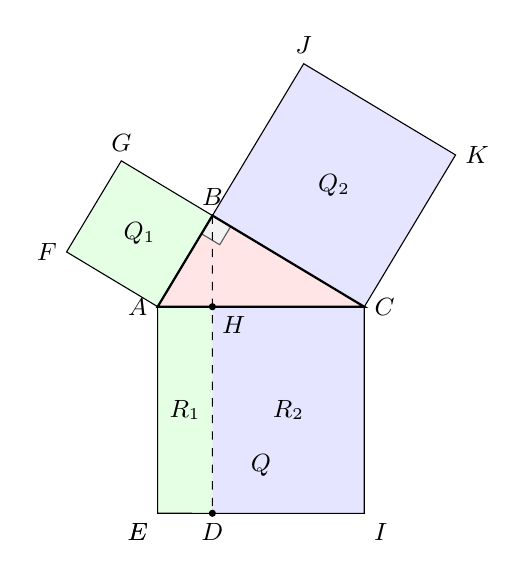
\begin{tikzpicture}[scale=0.9,font=\small]
\usetikzlibrary{calc}

%\begin{scope}[rotate=121]
\begin{scope}[rotate=-121]
\path[fill=red!10] (0,0) coordinate (a) -- (-1.5,0) coordinate (b) -- (-1.5,2.5) coordinate (c) -- cycle;
\draw[gray!70!black, fill=gray!10] (b) rectangle +(0.3,0.3);
\draw[fill=green!10] (a) let \p1=(b) in -- (b) -- (\x1,\x1) coordinate (g) node[above] {$G$} -- (0,\x1) coordinate (f) node [left] {$F$} -- cycle;
\draw[fill=blue!10] (b) let \p1=($(c)-(b)$) in -- (c) -- ++(-\y1,0) coordinate (k) node[right] {$K$} -- ++(0,-\y1) coordinate (j) node [above] {$J$} -- cycle;
\path (f) -- node {$Q_1$} (b);
\path (c) -- node {$Q_2$} (j);
\end{scope}
\coordinate (h) at ($(a)!(b)!(c)$);
\path[fill=green!10] (a) let \p1=(c) in -- (0,{-\x1}) coordinate (e) node[below left] {$E$} let \p2=(h) in -- +({\x2},0) coordinate (d) -- (h) -- cycle;
\path[fill=blue!10] (h) -- (c) let \p1=(c) in -- +(0,{-\x1}) coordinate (i) -- (d) -- cycle;

\draw (a) -- (e) node[below left] {$E$} -- (i) node[below right] {$I$} -- (c) -- cycle;
\draw[dashed] (b) -- (d);
\path (a) -- node {$R_1$} (d);
\path (d) -- node {$R_2$} (c);
\path (a) -- node[shift={(0,-0.7)}] {$Q$} (i);

\draw[thick] (a) node[left] {$A$} -- (b) node [above]{$B$} -- (c) node[right] {$C$} -- cycle;

\draw[fill] (h) circle (1.2pt) node[below right] {$H$};
\draw[fill] (d) circle (1.2pt) node[below] {$D$};
%\end{scope}

\end{tikzpicture}

\end{minipage}\vspace{8pt}


\begin{teorema}[Secondo teorema di Euclide]
In un triangolo rettangolo, il quadrato costruito sull'altezza 
relativa all'ipotenusa è equivalente al rettangolo che ha per 
dimensioni le proiezioni dei cateti sull'ipotenusa.
\end{teorema}

Dobbiamo dimostrare che il quadrato $Q$ che ha come lato l'altezza 
relativa all'ipotenusa è equivalente al rettangolo $R_1$ che ha come 
lati le due proiezioni dei cateti sull'ipotenusa.

\noindent\begin{minipage}{0.6\textwidth}\parindent15pt
\begin{proof}

La costruzione è la seguente: dopo aver disegnato il quadrato $Q$ si 
disegnano anche il quadrato $Q_1$, che ha come lato il cateto $AB$, 
ed il rettangolo $R$, che ha come lati l'ipotenusa e la proiezione 
$AH$ di $AB$ sull'ipotenusa. All'interno di questo rettangolo 
possiamo individuare il quadrato $Q_2$, di lato $AH$, ed il rettangolo 
$R_1$, che ha come dimensioni $NM\cong AH$ e $MD\cong HD-HM\cong HC$, 
in quanto $HD\cong AC$ e $HM\cong AH$.

Consideriamo ora il triangolo rettangolo $ABH$, e applichiamo ad esso 
il teorema di Pitagora, risulta $Q_1\doteq Q+Q_2$. Applichiamo ora al 
triangolo $ABC$ il primo teorema di Euclide, si ha $Q_1\doteq R$. 
Confrontiamo le due relazioni ed applichiamo la proprietà transitiva 
dell'equivalenza $Q+Q_2\doteq R$. Ma $R\doteq Q_2 + R_1$, quindi 
sostituendo avremo $Q+Q_2\doteq Q_2 + R_1$ e sottraendo ad ambo i 
membri la stessa quantità $Q_2$ otteniamo la tesi $Q\doteq R_1$.
\end{proof}
\end{minipage}\hfil
\begin{minipage}{0.4\textwidth}
  \centering% Copyright (c) 2015 Daniele Masini - d.masini.it@gmail.com

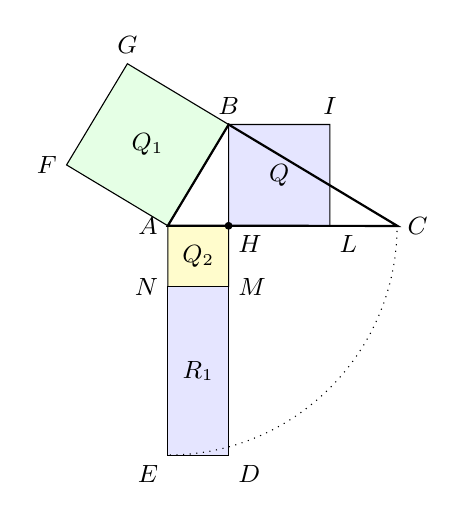
\begin{tikzpicture}[scale=1,font=\small]
\usetikzlibrary{calc}

%\begin{scope}[rotate=121]
\begin{scope}[rotate=-121]
\path (0,0) coordinate (a) -- (-1.5,0) coordinate (b) -- (-1.5,2.5) coordinate (c) -- cycle;
%\draw[gray!70!black, fill=gray!10] (b) rectangle +(0.3,0.3);
\draw[fill=green!10] (a) let \p1=(b) in -- (b) -- (\x1,\x1) coordinate (g) node[above] {$G$} -- (0,\x1) coordinate (f) node [left] {$F$} -- cycle;
\path (f) -- node {$Q_1$} (b);
\end{scope}
\coordinate (h) at ($(a)!(b)!(c)$);

\draw[fill=blue!10] (b) let \p1=($(b)-(h)$) in -- (h) -- ++({\y1},0) coordinate (l) node[below right] {$L$} -- ++(0,{\y1}) coordinate (i) node [above] {$I$} -- cycle;
\path (h) -- node {$Q$} (i);

\draw[fill=yellow!20] (a) -- (h) let \p1=(h) in -- ++(0,{-\x1}) coordinate (m) node[right] {$M$} -- +({-\x1},0) coordinate (n) node[left] {$N$} -- cycle;
\draw[fill=blue!10] (n) -- (m) let \p1=($(c)-(h)$) in -- ++(0,{-\x1}) coordinate (d) node[below right] {$D$} let \p2=(h) in -- +({-\x2},0) coordinate (e) node[below left] {$E$} -- cycle;

%\draw (a) -- (e) node[below left] {$E$} -- (i) node[below right] {$I$} -- (c) -- cycle;
%\draw[dashed] (b) -- (d);
\path (a) -- node {$Q_2$} (m);
\path (n) -- node {$R_1$} (d);
%\path (a) -- node {$Q$} (i);

\draw[thick] (a) node[left] {$A$} -- (b) node [above]{$B$} -- (c) node[right] {$C$} -- cycle;

\draw[fill] (h) circle (1.2pt) node[below right] {$H$};
\begin{scope}
\clip (a) -- (2.92,0) -- (2.92, -2.92) -- (0,-2.92) -- cycle;
\draw[dotted] (a) circle (2.912);
\end{scope}

\end{tikzpicture}

\end{minipage}\vspace{8pt}

Per ciascuno dei tre teoremi dimostrati vale anche il teorema inverso.

% \newpage %---------------------------------------------------

\section{Applicazioni dei teoremi di Euclide e Pitagora}
\label{sect:applicazioni_pitagora_euclide}

Consideriamo il triangolo rettangolo $ABC$ nella figura a fianco.
Supponiamo di conoscere la misura dell'ipotenusa $BC$ e della 
proiezione $CH$ del cateto $AC$, sull'ipotenusa; allora possiamo 
applicare il primo teorema di Euclide per trovare la lunghezza del 
cateto $AC$: $\overline{AC}^2=\overline{BC}\cdot \overline{CH}$, da 
cui si ricava $\overline{AC}=\sqrt{\overline{BC}\cdot \overline{CH}}$.

\begin{wrapfigure}{r}{0.25\textwidth}
  \centering% Copyright (c) 2015 Daniele Masini - d.masini.it@gmail.com

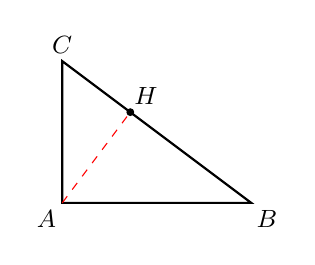
\begin{tikzpicture}[scale=1.2,font=\small]
\usetikzlibrary{calc}

\begin{scope}[xshift=2.5cm]

\draw[thick] (0,0) coordinate (a) node[shift={(-0.2,-0.2)}] {$A$} -- (2,0) coordinate (b) node[shift={(0.2,-0.2)}] {$B$} -- (0,1.5) coordinate (c) node[shift={(0,0.2)}] {$C$} -- cycle;

\draw[dashed, red] (a) -- ($(b)!(a)!(c)$) coordinate (h);

\draw[fill] (h) circle (1pt) node[black, shift={(0.2,0.2)}] {$H$};

\end{scope}


\end{tikzpicture}

  \caption{Esempi~\ref{es:7.4} e~\ref{es:7.5}}\label{fig:es7.4}
\end{wrapfigure}
Se invece conosciamo il cateto $AC$ e quella la sua 
proiezione $CH$ e vogliamo trovare l'ipotenusa, allora avremo 
$\overline{BC}=\dfrac{\overline{AC}^2}{\overline{CH}}$.

Supponiamo ora di conoscere le misure delle due proiezioni dei cateti 
sull'ipotenusa, $BH$ e $CH$, e di voler trovare la misura di $AH$, 
altezza relativa all'ipotenusa, applicando il secondo teorema di 
Euclide avremo $\overline{AH}^2=\overline{BH}\cdot \overline{CH}$, da 
cui si ricava $\overline{AH}=\sqrt{\overline{BH}\cdot\overline{CH}}$.

Se invece conosciamo l'altezza relativa all'ipotenusa ed una delle 
due proiezioni dei cateti, ad esempio $CH$, e vogliamo trovare la 
lunghezza dell'altra ($BH$), avremo 
$BH=\dfrac{\overline{AH}^2}{\overline{CH}}$.

Per quanto riguarda poi le applicazioni del teorema di Pitagora, che 
sicuramente lo studente conosce già dalle scuole medie, ricordiamo 
che se abbiamo la misura dei due cateti avremo 
$\overline{BC}^2=\overline{AB}^2+\overline{AC}^2$, da cui 
$\overline{BC}=\sqrt{\overline{AB}^2+\overline{AC}^2}$; viceversa, 
conoscendo l'ipotenusa ed un cateto, ad esempio $AC$, avremo 
$\overline{AB}=\sqrt{\overline{BC}^2-\overline{AC}^2}$.

% \begin{exrig}
\begin{esempio}\label{es:7.4}
Calcolare perimetro ed area di un triangolo rettangolo che ha un 
cateto lungo 10~cm e la sua proiezione sull'ipotenusa lunga 
8~cm.\vspace{7pt}

Facendo riferimento alla figura~\ref{fig:es7.4}, 
$\overline{AC}=10$~cm, $\overline{CH}=8$~cm.

Applichiamo il primo teorema di Euclide per trovare la lunghezza 
dell'ipotenusa 
$\overline{BC}=\dfrac{\overline{AC}^2}{\overline{CH}}=\dfrac{10^2}{8}
=\dfrac{100}{8}=\np{12,5}$~cm. Per trovare l'altro cateto possiamo 
applicare il teorema di Pitagora 
$\overline{AB}=\sqrt{\overline{BC}^2-\overline{AC}^2}=\sqrt{\dfrac{625
}{4}-100}=\sqrt{\dfrac{225}{4}}=\dfrac{15}{2}=\np{7,5}$~cm.
Quando il teorema di Pitagora viene applicato per trovare un cateto 
si può anche semplificare il calcolo scomponendo la differenza di 
quadrati
\begin{align*}
\overline{AB}&=\sqrt{\overline{BC}^2-\overline{AC}^2}=\sqrt{(\overline
{BC}-\overline{AC})\cdot(\overline{BC}+\overline{AC})}=\sqrt{
\left(\dfrac{25}{2}-10\right)\cdot\left(\dfrac{25}{2}+10\right)}=\sqrt
{\dfrac{5}{2}\cdot\dfrac{45}{2}}\\
&=\sqrt{\dfrac{5^2\cdot 3^2}{2^2}}=\dfrac{5\cdot 
3}{2}=\dfrac{15}{2}=\np{7,5}\text{~cm.}
\end{align*}

A questo punto conosciamo tutti i lati, quindi possiamo calcolare il 
perimetro $2p=8+\np{7,5}+\np{12,5}=30$~cm e l'area 
$A=(\text{cateto}\times\text{cateto})/2 = 
\np{37,5}$~cm\textsuperscript{2}.
\end{esempio}

% \begin{inaccessibleblock}[Figura: TODO]
%  \begin{figure}[!htb]
%   \centering% Copyright (c) 2015 Daniele Masini - d.masini.it@gmail.com

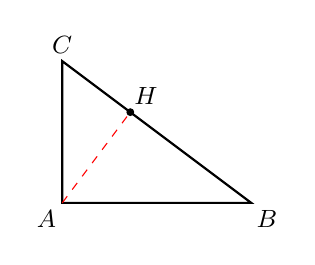
\begin{tikzpicture}[scale=1.2,font=\small]
\usetikzlibrary{calc}

\begin{scope}[xshift=2.5cm]

\draw[thick] (0,0) coordinate (a) node[shift={(-0.2,-0.2)}] {$A$} -- (2,0) coordinate (b) node[shift={(0.2,-0.2)}] {$B$} -- (0,1.5) coordinate (c) node[shift={(0,0.2)}] {$C$} -- cycle;

\draw[dashed, red] (a) -- ($(b)!(a)!(c)$) coordinate (h);

\draw[fill] (h) circle (1pt) node[black, shift={(0.2,0.2)}] {$H$};

\end{scope}


\end{tikzpicture}

%   \caption{Esempi~\ref{es:7.4} e~\ref{es:7.5}}\label{fig:es7.4}
% \end{figure}
% \end{inaccessibleblock}

\begin{esempio}\label{es:7.5}

Nel triangolo rettangolo $ABC$ (figura~\ref{fig:es7.4})l'altezza relativa 
all'ipotenusa misura 12~cm. 
Il perimetro del triangolo formato dall'altezza e da uno 
dei cateti è 36~cm. Determina la proiezione dell'altro cateto 
sull'ipotenusa e il perimetro del triangolo $ABC$.\vspace{7pt}

% \begin{minipage}{.69 \textwidth}
% Nel triangolo rettangolo $ABC$ l'altezza relativa all'ipotenusa 
% misura 12~cm. Il perimetro del triangolo formato dall'altezza e da uno 
% dei cateti è 36~cm. Determina la proiezione dell'altro cateto 
% sull'ipotenusa e il perimetro del triangolo $ABC$.\vspace{7pt}
% \end{minipage}
% \hfill
% \begin{minipage}{.29 \textwidth}
% \begin{inaccessibleblock}[Triangolo rettangolo con indicata l'altezza AH 
% relativa all'ipotenusa BC]
% \centering% Copyright (c) 2015 Daniele Masini - d.masini.it@gmail.com

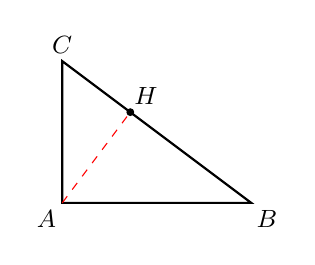
\begin{tikzpicture}[scale=1.2,font=\small]
\usetikzlibrary{calc}

\begin{scope}[xshift=2.5cm]

\draw[thick] (0,0) coordinate (a) node[shift={(-0.2,-0.2)}] {$A$} -- (2,0) coordinate (b) node[shift={(0.2,-0.2)}] {$B$} -- (0,1.5) coordinate (c) node[shift={(0,0.2)}] {$C$} -- cycle;

\draw[dashed, red] (a) -- ($(b)!(a)!(c)$) coordinate (h);

\draw[fill] (h) circle (1pt) node[black, shift={(0.2,0.2)}] {$H$};

\end{scope}


\end{tikzpicture}
 \label{fig:es7.4}
% \end{inaccessibleblock}
% \end{minipage}

Dai dati si ha che $AH = 12$~cm, e $2p_{ABH} = 36$~cm 
(figura~\ref{fig:es7.4}).
Questo vuol dire che $AB + BH = 2p - AH = 24$~cm. 
Posso allora porre $AB = x$, da cui $BH = 24 – x$.
Applichiamo il teorema di Pitagora ed otteniamo l'equazione
\[x^2 = 12^2 + (24 - x)^2 \quad\Rightarrow\quad x^2 = 12^2 + 24^2 - 
48x + x^2\]
sviluppando i calcoli, il termine in $x^2$ si elimina e otteniamo 
l'equazione di primo grado $48x = 24^2 + 12^2$.
Per evitare i calcoli raccogliamo al secondo membro $12^2$, quindi 
ricaviamo $x=\dfrac{12^2\cdot\left(2^2+1\right)}{4\cdot 12}=15$~cm.

A questo punto possiamo ottenere $BH = 24-x = 24-15 = 9$~cm. Oppure, 
ricorrendo alla terna pitagorica fondamentale 3, 4, 5, di cui i lati 
del triangolo $ABH$ sono multipli secondo il numero 3, ho $BH = 3 
\cdot 3 = 9$~cm.

Per ricavare $CH$ applichiamo il secondo teorema di Euclide 
$\overline{CH}=\dfrac{\overline{AH}^2}{\overline{BH}}=\dfrac{144}{9}
=16$~cm.

Sommando $CH$ con $BH$ troviamo l'ipotenusa $BC=25$~cm. Per ricavare 
l'altro cateto ricorriamo alla terna pitagorica fondamentale 
$AB=3\cdot 5=15$~cm, $BC=5\cdot 5=25$~cm, da cui $AC=4\cdot 5=20$~cm.
Il perimetro vale quindi $2p=15+25+20=60$~cm.
\end{esempio}
% \end{exrig}

\section{Applicazioni dell'algebra alla geometria}
\label{sect:applicazioni_algebra}

\subsection{Triangoli rettangoli con angoli di 45°}

\begin{wrapfigure}{r}{0.20\textwidth}
  \centering% Copyright (c) 2015 Daniele Masini - d.masini.it@gmail.com

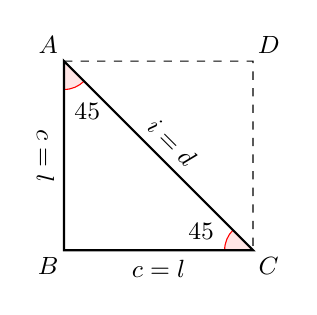
\begin{tikzpicture}[scale=1.2,font=\small]
\usetikzlibrary{calc}

\begin{scope}

\path (0,0) coordinate (b) -- (2,0) coordinate (c) -- (0,2) coordinate (a) -- cycle;

\draw[dashed] (a) -- (2,2) coordinate (d) node[shift={(0.2,0.2)}] {$D$} -- (c);

\begin{scope}
\clip (a) -- (b) -- (c) -- cycle;
\draw[red, fill=red!10] (a) circle (0.3) node[black, shift={(-65:0.7)}] {$45\grado$};
\draw[red, fill=red!10] (c) circle (0.3) node[black, shift={(160:0.7)}] {$45\grado$};
\end{scope}

\draw[thick] (b) node[shift={(-0.2,-0.2)}] {$B$} -- node[below] {$c=l$} (c) node[shift={(0.2,-0.2)}] {$C$} -- node[above, midway, sloped] {$i=d$} (a) node[shift={(-0.2,0.2)}] {$A$} -- cycle;

\path (a) -- node[below, midway, sloped] {$c=l$} (b);

\end{scope}


\end{tikzpicture}

\end{wrapfigure}
Un triangolo rettangolo avente un angolo di $45\grado$ è 
necessariamente isoscele, in quanto anche il terzo angolo varrà 
$45\grado$, infatti $180\grado - (90\grado+45\grado)=45\grado$.
Indicando con $i$ l'ipotenusa e con $c$ ognuno dei due cateti, 
applicando il teorema di Pitagora avremo 
$i=\sqrt{c^2+c^2}=\sqrt{2c^2}=c\sqrt{2}$.

Viceversa, se conosciamo l'ipotenusa e vogliamo ricavare i cateti, 
passando alla formula inversa e razionalizzando avremo 
$c=\dfrac{i}{\sqrt{2}}=i\dfrac{\sqrt{2}}{2}$.

Un triangolo rettangolo isoscele può anche essere interpretato come 
metà di un quadrato, di cui i cateti sono i lati e l'ipotenusa è la 
diagonale.
Indicando con $l$ il lato e $d$ la diagonale, anche per un quadrato 
varranno quindi le precedenti relazioni, ovvero $d=l\sqrt{2}$ e 
$l=d\dfrac{\sqrt{2}}{2}$.

% \newpage %---------------------------------------------------

\subsection{Triangoli rettangoli con angoli di 30° e 60°}

\begin{wrapfigure}{r}{0.25\textwidth}
  \centering% Copyright (c) 2015 Daniele Masini - d.masini.it@gmail.com


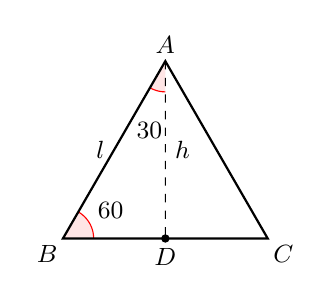
\begin{tikzpicture}[scale=1.3,font=\small]
\usetikzlibrary{calc}

\begin{scope}

\path (0,0) coordinate (b) -- (2,0) coordinate (c) -- ++(120:2) coordinate (a) -- cycle;

\coordinate (d) at ($(b)!(a)!(c)$);

\begin{scope}
\clip (a) -- (d) -- (b) -- cycle;
\draw[red, fill=red!10] (a) circle (0.3) node[black, shift={(257:0.9)}] {$30\grado$};
\draw[red, fill=red!10] (b) circle (0.3) node[black, shift={(30:0.7)}] {$60\grado$};
\end{scope}

\draw[dashed] (a) -- node[right] {$h$} (d) node[below] {$D$};

\draw[thick] (b) node[shift={(-0.2,-0.2)}] {$B$} -- (c) node[shift={(0.2,-0.2)}] {$C$} -- (a) node[shift={(0,0.2)}] {$A$} -- cycle;

\path (a) -- node[left] {$l$} (b);

\draw[fill] (d) circle (1pt);

\end{scope}


\end{tikzpicture}
\end{wrapfigure}
Un triangolo rettangolo con un angolo di $30\grado$ avrà il secondo 
angolo acuto di $60\grado$, infatti $180\grado- 
(90\grado+30\grado)=60\grado$. Questo triangolo può essere 
interpretato come metà di un triangolo equilatero: l'ipotenusa 
coincide con il lato di questo triangolo, il cateto adiacente 
all'angolo di $60\grado$ è metà del lato del triangolo equilatero ed 
il cateto adiacente all'angolo di $30\grado$ è l'altezza del 
triangolo equilatero.
Dunque, indicando con $i$ l'ipotenusa, il cateto $BD$, adiacente 
all'angolo di $60\grado$, varrà $\dfrac{i}{2}$, mentre il cateto 
$AD$, opposto all'angolo di $60\grado$ e adiacente a quello di 
$30\grado$, applicando il teorema di Pitagora, varrà 
$AD=\sqrt{i^2-\left(\dfrac{i}{2}\right)^2}=\sqrt{i^2-\dfrac{i^2}{4}}
=\sqrt{\dfrac{3i^2}{4}}=i\dfrac{\sqrt{3}}{2}$.

Viceversa, se conosciamo il cateto $AD$ e vogliamo ricavare 
l'ipotenusa, passando alla formula inversa e razionalizzando avremo 
$i=\dfrac{2AD}{\sqrt{3}}=2AD\dfrac{\sqrt{3}}{3}$.

Indicando quindi con $l$ il lato del triangolo equilatero e con $h$ 
la sua altezza avremo analogamente $h=l\dfrac{\sqrt{3}}{2}$ e 
$l=2h\dfrac{\sqrt{3}}{3}$.

In questo modo possiamo anche determinare l'area di un qualunque 
triangolo equilatero conoscendone soltanto il lato $A=\dfrac{b\cdot 
h}{2}=\dfrac{1}{2}\cdot l\cdot 
l\dfrac{\sqrt{3}}{2}=l^2\dfrac{\sqrt{3}}{4}$.

% \begin{exrig}
\begin{esempio}\label{es:7.6}
Gli angoli adiacenti alla base minore di un trapezio isoscele 
misurano $135\grado$. Determinare area e perimetro del trapezio, 
sapendo che le basi misurano 4~cm e 20~cm.\vspace{7pt}

Tracciamo l'altezza $AH$ (figura~\ref{fig:es7.6}); si verrà così a 
determinare il triangolo rettangolo $ABH$. Poiché 
$A\widehat{B}H=45\grado$, anche $B\widehat{A}H=45\grado$. Avremo 
quindi $\overline{BH}=\overline{AH}$; ma 
$\overline{BH}=\dfrac{\overline{BC}-\overline{AD}}{2}=8$~cm, quindi 
$\overline{AH}=8$~cm. L'area vale dunque $A=\dfrac{(20+4)\cdot 
8}{2}=96$~cm\textsuperscript{2}.

Per calcolare il perimetro ricordiamo che 
$\overline{AB}=\overline{BH}\sqrt{2}=8\sqrt{2}$~cm e 
$\overline{CD}=\overline{AB}$.
Dunque $2p=20+4+2\cdot 8\sqrt{2}=24+16\sqrt{2}=8(3+2\sqrt{2})$~cm.
\end{esempio}

\vspace{-2em}

\begin{inaccessibleblock}[Figura: TODO]
 \begin{figure}[!htb]
  \begin{center}
    \begin{minipage}{0.45\textwidth}
      \centering
      % Copyright (c) 2015 Daniele Masini - d.masini.it@gmail.com

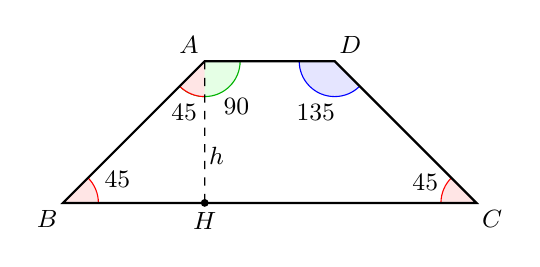
\begin{tikzpicture}[scale=1.5,font=\small]
\usetikzlibrary{calc}

\begin{scope}

\path (0,0) coordinate (b) -- (3.5,0) coordinate (c) -- (2.3,1.2) coordinate (d) -- (1.2,1.2) coordinate (a) -- cycle;

\coordinate (h) at ($(b)!(a)!(c)$);

\begin{scope}
\clip (a) -- (b) -- (c) -- (d) -- cycle;
\draw[green!70!black, fill=green!10] (a) circle (0.3) node[black, shift={(305:0.7)}] {$90\grado$};
\draw[blue, fill=blue!10] (d) circle (0.3) node[black, shift={(250:0.7)}] {$135\grado$};
\draw[red, fill=red!10] (b) circle (0.3) node[black, shift={(23:0.75)}] {$45\grado$};
\draw[red, fill=red!10] (c) circle (0.3) node[black, shift={(158:0.7)}] {$45\grado$};
\end{scope}

\begin{scope}
\clip (a) -- (b) -- (h) -- cycle;
\draw[red, fill=red!10] (a) circle (0.3) node[black, shift={(248:0.7)}] {$45\grado$};
\end{scope}

\draw[dashed] (a) -- node[shift={(0.15,-0.3)}] {$h$} (h) node[below] {$H$};

\draw[thick] (b) node[shift={(-0.2,-0.2)}] {$B$} -- (c) node[shift={(0.2,-0.2)}] {$C$} -- (d) node[shift={(0.2,0.2)}] {$D$} -- (a) node[shift={(-0.2,0.2)}] {$A$} -- cycle;

\draw[fill] (h) circle (.8pt);

\end{scope}


\end{tikzpicture}

      
\caption{Esempio~\ref{es:7.6}}\label{fig:es7.6}
    \end{minipage}
    \hspace{0.03\textwidth}  
    \begin{minipage}{0.45\textwidth}
      \centering
      % Copyright (c) 2015 Daniele Masini - d.masini.it@gmail.com

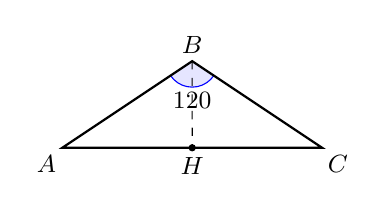
\begin{tikzpicture}[scale=1.1,font=\small]
\usetikzlibrary{calc}

\begin{scope}

\path (0,0) coordinate (a) -- (1.5,1) coordinate (b) -- (3,0) coordinate (c) -- cycle;

\coordinate (h) at ($(a)!(b)!(c)$);

\begin{scope}
\clip (a) -- (b) -- (c) -- cycle;
\draw[blue, fill=blue!10] (b) circle (0.3) node[black, shift={(270:0.5)}] {$120\grado$};
\end{scope}

\draw[dashed] (b) -- (h) node[below] {$H$};

\draw[thick] (a) node[shift={(-0.2,-0.2)}] {$A$} -- (b) node[shift={(0,0.2)}] {$B$} -- (c) node[shift={(0.2,-0.2)}] {$C$} -- cycle;

\draw[fill] (h) circle (1pt);

\end{scope}

\end{tikzpicture}

      
\caption{Esempio~\ref{es:7.7}}\label{fig:es7.7}
    \end{minipage}
  \end{center}
\end{figure}
\end{inaccessibleblock}

\vspace{-3em}

\begin{esempio}\label{es:7.7}
Un triangolo isoscele ha l'angolo al vertice di $120\grado$. 
Determina perimetro ed area sapendo che la base è lunga 
60~cm.\vspace{7pt}

Tracciamo l'altezza $BH$ (figura~\ref{fig:es7.7}). Poiché il 
triangolo è isoscele, l'altezza relativa alla base è anche mediana, 
quindi $AH\cong HC$; ma $BH$ è anche bisettrice dell'angolo al vertice 
$B$, quindi si ottengono due triangoli rettangoli tra loro 
congruenti, ciascuno dei quali ha in $B$ un angolo di $60\grado$. 
Consideriamo uno dei due triangoli, ad esempio $ABH$; il cateto 
$\overline{AH}=30$~cm; poiché l'angolo $\widehat{A}=30\grado$, per 
calcolare $\overline{AB}$ si deve usare la formula inversa 
$\overline{AB}=\dfrac{2\overline{AH}\sqrt{3}}{3}=\dfrac{2\cdot 
30\sqrt{3}}{3}=20\sqrt{3}$~cm.
Il perimetro vale dunque $2p=60 + 40\sqrt{3} = 20 (3 + 2\sqrt{3})$~cm.

Per calcolare l'area bisogna prima trovare $\overline{BH}$, che è 
congruente a metà ipotenusa $\overline{BH}=10\sqrt{3}$~cm. Quindi 
$A=\dfrac{60\cdot 10\sqrt{3}}{2}=300\sqrt{3}$~cm\textsuperscript{2}.
\end{esempio}
% \end{exrig}

\subsection{Formula di Erone per il calcolo dell'area di un triangolo}

La \emph{formula di Erone} permette di calcolare l'area di un 
triangolo qualsiasi se si conoscono le misure dei suoi lati.

\begin{wrapfigure}{r}{0.3\textwidth}
        \centering% Copyright (c) 2015 Daniele Masini - d.masini.it@gmail.com

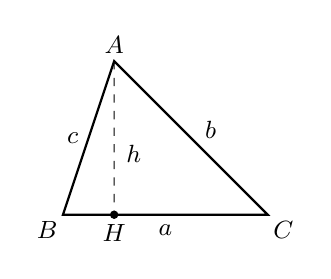
\begin{tikzpicture}[scale=1.3,font=\small]
\usetikzlibrary{calc}

\begin{scope}

\path (0,0) coordinate (b) -- (2,0) coordinate (c) -- (0.5,1.5) coordinate (a) -- cycle;

\coordinate (h) at ($(b)!(a)!(c)$);

\draw[dashed] (a) -- node[shift={(0.25,-0.2)}] {$h$} (h) node[below] {$H$};

\draw[thick] (a) node[shift={(0,0.2)}] {$A$} -- node[left] {$c$} (b) node[shift={(-0.2,-0.2)}] {$B$} -- node[below] {$a$} (c) node[shift={(0.2,-0.2)}] {$C$} -- cycle;

\draw[fill] (h) circle (1pt);
\path (c) -- node[shift={(0.25,0.1)}] {$b$} (a);

\end{scope}


\end{tikzpicture}

        \vspace{10pt}
\end{wrapfigure}

La sua dimostrazione è piuttosto complicata e non verrà presentata qui, ma la 
formula può essere utile in alcune circostanze:
\[A=\sqrt{p(p-a)(p-b)(p-c)}\]
Dove con \(p\) si intende il semiperimetro:
\[p= \dfrac{a+b+c}{2}\]

\begin{comment}
\subsection{Formula di Erone per il calcolo dell'area di un triangolo}

La \emph{formula di Erone} permette di calcolare l'area di un 
triangolo qualsiasi se si conoscono le misure dei suoi lati.
Vediamo la dimostrazione nel caso di un triangolo acutangolo. 
Con analoga procedura si può dimostrare per un qualsiasi tipo di triangolo.

\begin{wrapfigure}{r}{0.3\textwidth}
  \centering% Copyright (c) 2015 Daniele Masini - d.masini.it@gmail.com

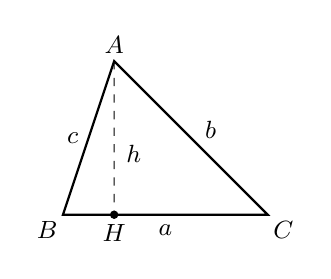
\begin{tikzpicture}[scale=1.3,font=\small]
\usetikzlibrary{calc}

\begin{scope}

\path (0,0) coordinate (b) -- (2,0) coordinate (c) -- (0.5,1.5) coordinate (a) -- cycle;

\coordinate (h) at ($(b)!(a)!(c)$);

\draw[dashed] (a) -- node[shift={(0.25,-0.2)}] {$h$} (h) node[below] {$H$};

\draw[thick] (a) node[shift={(0,0.2)}] {$A$} -- node[left] {$c$} (b) node[shift={(-0.2,-0.2)}] {$B$} -- node[below] {$a$} (c) node[shift={(0.2,-0.2)}] {$C$} -- cycle;

\draw[fill] (h) circle (1pt);
\path (c) -- node[shift={(0.25,0.1)}] {$b$} (a);

\end{scope}


\end{tikzpicture}

  \vspace{10pt}
\end{wrapfigure}
Sia $a$ la misura del lato $BC$ e sia $H$ il piede dell'altezza $h$ 
del triangolo rispetto a $BC$. Ponendo $BH = x$ si avrà $HC = a - x$.
Dal teorema di Pitagora si ha
\begin{equation}\label{eq:7.1}
h^2=c^2-x^2
\end{equation}
ma anche
\[h^2=b^2-(a-x)^2.\]

Uguagliamo le due espressioni e svolgiamo i calcoli. Otteniamo
\[c^2-x^2=b^2-a^2+2ax-x^2\]
da cui
\[x=\dfrac{c^2+a^2-b^2}{2a}.\]

Sostituendo questo valore di $x$ nella~(\ref{eq:7.1}), otteniamo
\[h^2=c^2-\left(\dfrac{c^2+a^2-b^2}{2a}\right)=\dfrac{
4a^2c^2-\left(c^2+a^2-b^2\right)^2}{4a^2}.\]

Poiché il numeratore è una differenza di quadrati possiamo scomporlo 
ottenendo
\begin{align*}
h^2&=\dfrac{\left[2ac-\left(c^2+a^2-b^2\right)\right]\cdot\left[
2ac+\left(c^2+a^2-b^2\right)\right]}{4a^2}\\
&=\dfrac{\left[2ac-c^2-a^2+b^2\right]\cdot\left[2ac+c^2+a^2-b^2\right]
}{4a^2}\\
&=\dfrac{\left[b^2-(a-c)^2\right]\cdot\left[(a+c)^2-b^2\right]}{4a^2}.
\end{align*}

Abbiamo ottenuto nuovamente delle differenze di quadrati che possiamo 
ulteriormente scomporre
\[h^2=\dfrac{(b+a-c)\cdot(b-a+c)\cdot(a+c+b)\cdot(a+c-b)}{4a^2}.\]
Al numeratore abbiamo
\[a + c + b = 2p\]
\[b + a - c = b+a+c-2c = 2p-2c = 2(p-c)\]
\[b - a + c = 2p - 2a = 2 (p - a)\]
\[a + c - b = 2p - 2b = 2(p - b)\]
quindi
\begin{align*}
h&=\sqrt{\dfrac{2p\cdot 2(p-a) \cdot 2(p-b) \cdot 
2(p-c)}{4a^2}}=\sqrt{\dfrac{16p\cdot (p-a) \cdot (p-b) \cdot 
(p-c)}{4a^2}}\\
&=\dfrac{2}{a}\sqrt{p(p-a)(p-b)(p-c)}.
\end{align*}

Infine calcoliamo l'area, ottenendo così la formula di Erone

\noindent{\begin{center} $A=\dfrac{1}{2}a\cdot h= 
\dfrac{1}{\cancel{2}}\cancel{a}\cdot\dfrac{\cancel{2}}{\cancel{a}}
\sqrt{p(p-a)(p-b)(p-c)} \:\Rightarrow$ 
\fbox{$A=\sqrt{p(p-a)(p-b)(p-c)}$}.\end{center}}
\end{comment}

% \begin{empheq}[box=\fbox]{equation*}
% A=\dfrac{1}{2}a\cdot h= 
% \dfrac{1}{\cancel{2}}\cancel{a}\cdot\dfrac{\cancel{2}}{\cancel{a}}
% \sqrt{p(p-a)(p-b)(p-c)}=\sqrt{p(p-a)(p-b)(p-c)}.
%\end{empheq}


% \setlength{\intextsep}{\defintextsep}
% 
% \newpage
% 
% \input{./chap/07_esercizi}
% 
% \cleardoublepage
